\graphicspath{{chapters/03/images/}}
\chapter{Implementation of the Stochastic Simulation Algorithms}

\section{Introduction}

  \subsection{Non-deterministic vs stochastic}
  Working under the assumption of using the same model and parameters:

  \begin{multicols}{2}
    \begin{itemize}
      \item A deterministic system does not show randomness and the same result is always obtained.
      \item A non-deterministic system shows some degree of uncertainty: different runs have different results.
    \end{itemize}
  \end{multicols}

    \subsubsection{Exact stochastic simulation}
    In an exact stochastic simulation, if some hypotheses are satisfied the system will behave like the biological one.
    Although the probability function could be computed, this does not make the method deterministic: uncertainty is intrinsic in the model.
    Theoretically there is no insight on the execution of the reactions in a stochastic setting, but a high level of accuracy can be reached thanks to the probability function.

  \subsection{Advantages of a non-deterministic approach}
  The reasoning behind the employment of a non-deterministic approach lies in the fact that to model a biological system there is a need to compromise between time and complexity.
  In non-deterministic polynomial time algorithms don't have an efficient solution, but it seems possible to find it.
  A non-deterministic setting allows us to understand whether an algorithm can be solved in polynomial time by step-wise guessing.

  \subsection{Categories of the exact simulation algorithms}
  A summary of the main exact stochastic simulation algorithms is reported in figure \ref{fig:tree}.

  \begin{figure}[H]
    \centering
    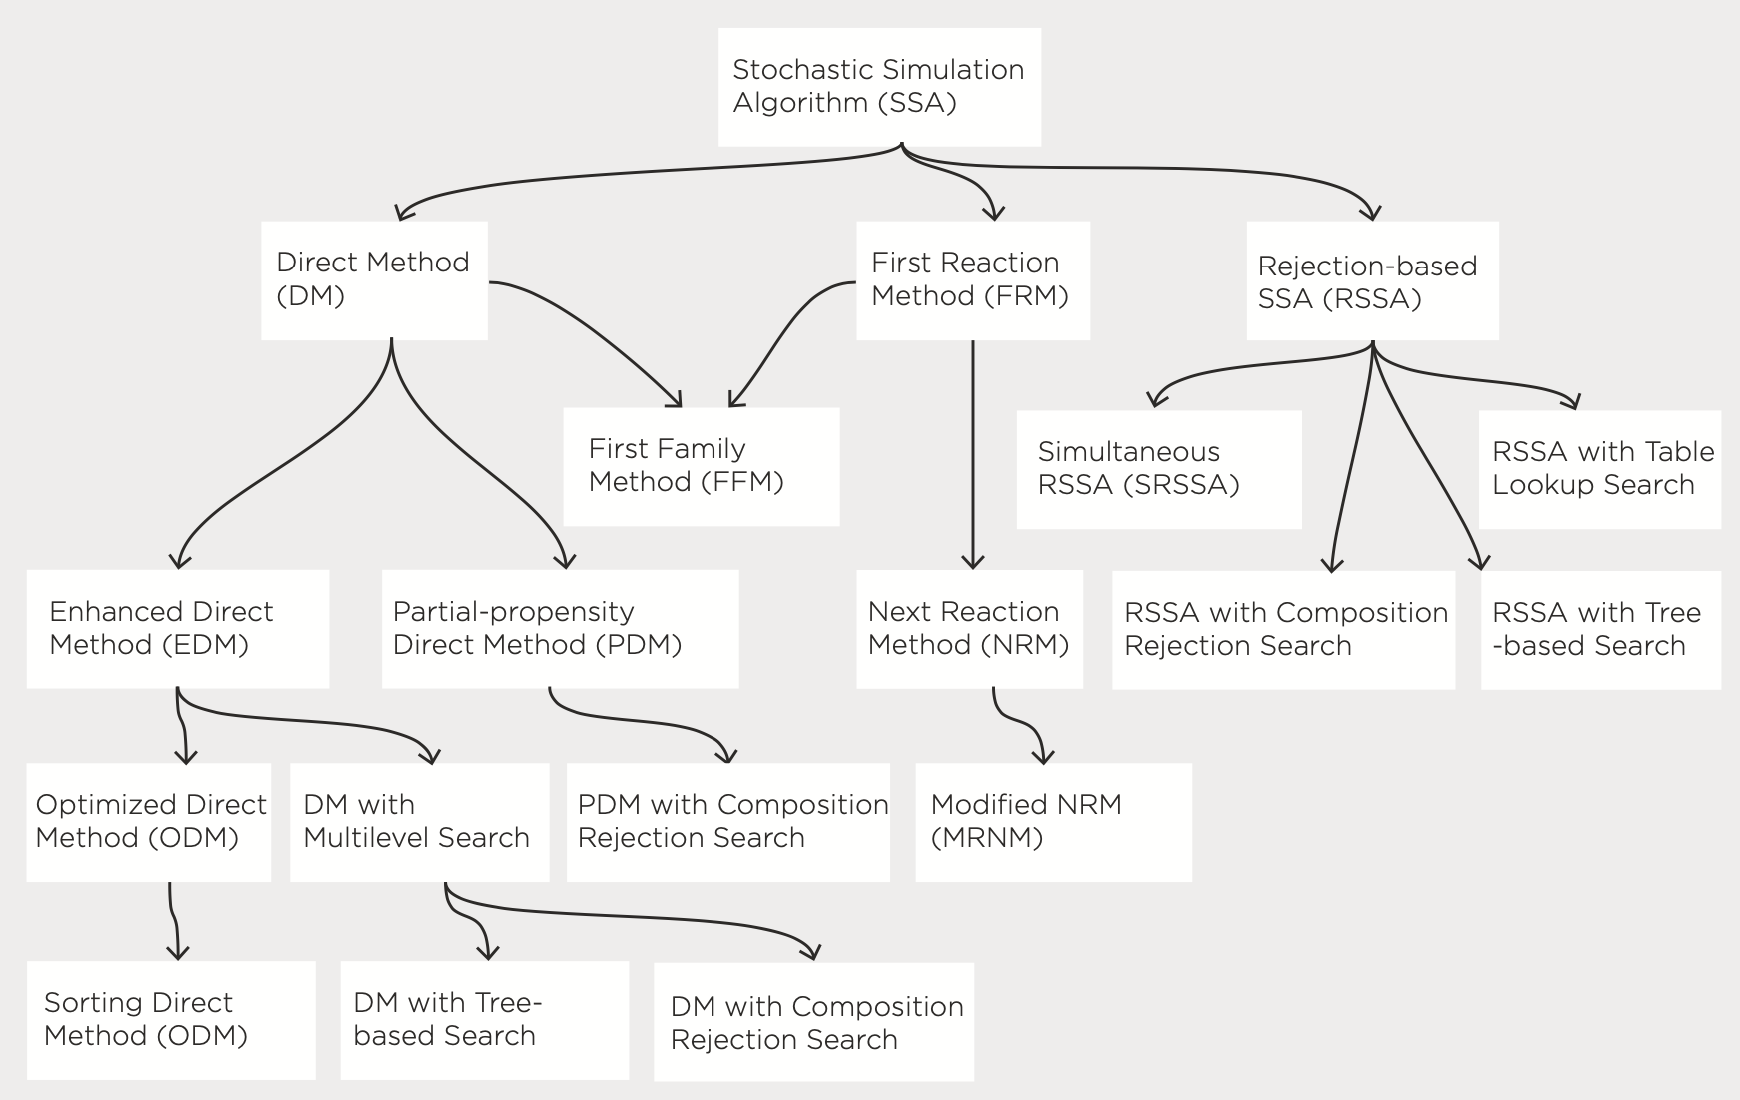
\includegraphics[width=\textwidth]{tree_methods.png}
    \caption{Main stochastic simulation algorithm.}
    \label{fig:tree}
  \end{figure}

\section{Direct method}
Gillespie's direct method defines a couple of formulae able to understand how the system will execute in terms of time $\tau$ and reactions $\mu$.
Since each time step is infinitesimal each reaction occurs and ends exactly at time $\tau$, hence there cannot be multiple reactions firing simultaneously.
Let $a_0$ be the sum of all propensities in the system, then the algorithm works as follow:

\begin{enumerate}
  \item Sample one random number from the distribution $a_0 = \sum_{j=1}^{M}{a_j}\rightarrow V_1=U(0,1)$.
  \item Scale it to the maximum $V_1 \cdot a_0 =U(0,a_0)$.
  \item See where this number will point over the different propensities ( Figure \ref{fig:boundaries}).

    \begin{figure}[H]
      \centering
      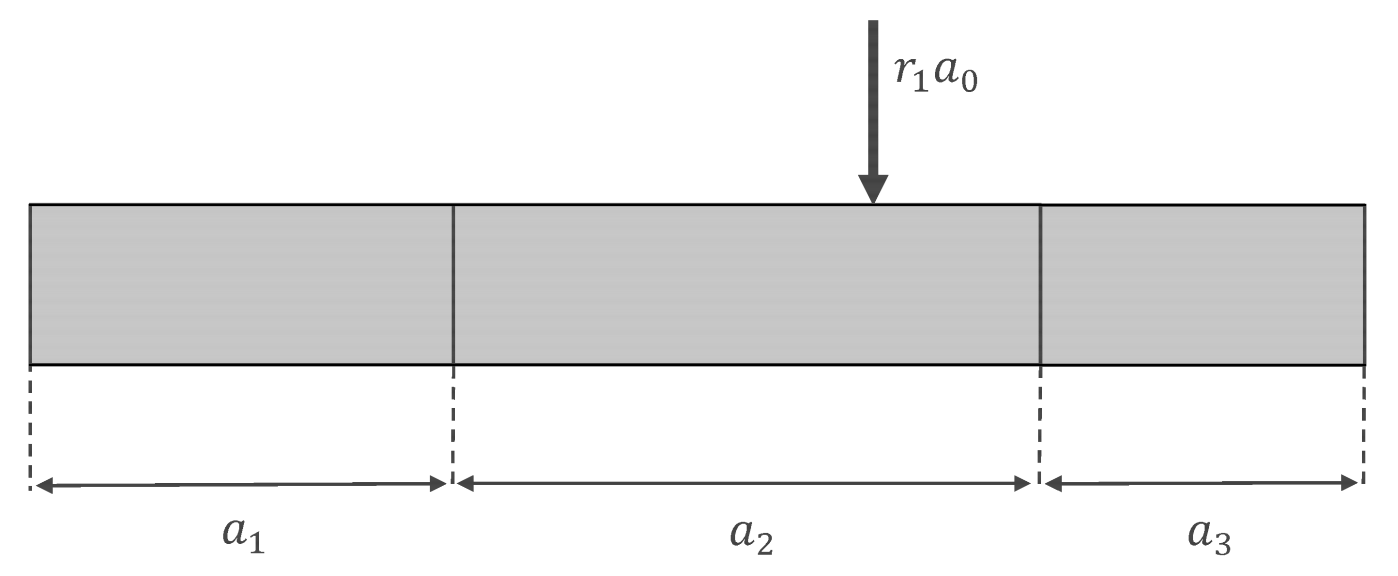
\includegraphics[width=\textwidth]{boundaries.png}
      \caption{Boundaries on the propensities.}
      \label{fig:boundaries}
    \end{figure}

  \item Generate another random number $V_2 =U(0,1)$ \item $\tau \sim Exp(a_0)$ \item $\tau = \frac{1}{a_0}ln(\frac{1}{V_2})$.
\end{enumerate}

  \subsection{Mathematical discussion}
  Gillespie's direct method is used to sample the pdf $p(\tau, \mu|\vec{x},t)$.
  The direct method partitions the joint probability density function into the product of two one-variable probability functions, one for $\tau$ and one for $\mu$ that can be sampled independently.
  The pdf can be factorized by the chain rule of probability as:

  $$p(\tau, \mu|\vec{x},t) = p_1(\tau|\vec{x},t)p_2(\mu|\vec{x},t)$$

  Where:

  \begin{multicols}{2}
    \begin{itemize}
      \item $p_1$ is the probability density function of the firing time $\tau$.
      \item $p_2$ is the probability density function of the reaction with index $\mu$ that fires at $t+\tau$.
    \end{itemize}
  \end{multicols}

  So that $p_1(\tau|\vec{x},t)d\tau$ is the probability that a reaction will fire in the next time interval $[t+\tau, t+\tau+d\tau[$.
  This marginal probability is obtained by summing the probability $p(\tau, \mu|\vec{x},t)d\tau$ over the domain of all possible values of reaction index $\mu$:

  $$p(\tau|\vec{x},t) = \sum\limits_{\mu=1}^Mp(\tau, \mu|\vec{x},t) = \sum\limits_{\mu=1}^Ma_\mu e^{a_0\tau} = a_0e^{-a_0\tau}$$

  Where $a_0$ is the total propensity.
  Plugging this and recalling the formula of the joint pdf:

  $$p_2(\mu|\tau,\vec{x},t) = \frac{p(\tau,\mu|\vec{x},t)}{p_1(\tau|\vec{x},t)} = \frac{a_\mu}{a_0}$$

  It can be seen how $p_2$ is independent of $\tau$, so it can be written as:

  $$p_2(\mu|\vec{x},t) = p_2(\mu|\tau,\vec{x},t) = \frac{a_\mu}{a_0}$$

  To verify that these two equation are part of the pdf:

  $$\int_0^{\infty}p_1(\tau|\vec{x},t)d\tau = \int_0^{\infty}a_0e^{-a_0\tau}d\tau = 1 \qquad\land\qquad \sum\limits_{\mu=1}^Mp_2(\mu|\vec{x},t) = \sum\limits_{\mu=1}^M\frac{a_\mu}{a_0} = 1$$

  The direct method uses $p_1(\tau|\vec{x},t)$ to sample the firing time $\tau$ and $p_2(\mu|\vec{x},t)$ to sample the reaction index $\mu$.
  Since the two pdfs are independent the firing time and the reaction index can be sampled independently, so that the order of sampling does not effect the exactness of the direct method.
  The generated firing time $\tau$ and the next reaction firing $R_\mu$ are ensured to have the pdf $p(\tau,\mu|\vec{x},t)$ specified by the stochastic simulation algorithm, so that the generated trajectories are exact.

    \subsubsection{Choice of the reaction}
    The selection of the next reaction index $\mu$ has probability $\frac{a_\mu}{a_0}$.
    Given $M$ discrete probabilities $\frac{a_j}{a_0}$ with $j = 1,\dots, M$, the choice of the next reaction index:

    \begin{align*}
      \mu &= \arg\min\limits_{\mu\in j=1,\dots,M}\sum\limits_{j=1}^M\frac{a_j}{a_0}\ge r_1 =\\
        &= \arg\min\limits_{\mu\in j=1,\dots,M}\sum\limits_{j=1}^Ma_j\ge r_1a_0
    \end{align*}

    Where $r_1$ is a uniformly distributed random number $norm(0,1)$.
    To select the next reaction firing $R_\mu$, the direct methods accumulates the sum $\sum\limits_{j=1}^\mu a_j$ until it finds the smallest index $\mu$ that satisfies that inequality.

    \subsubsection{Selection of the firing time}
    For the reaction of the firing time $\tau$, consider its pdf $p_1(\tau|\vec{x},t)$.
    It can be noted ho it is an exponential distribution with rate $a_0$.
    So the firing time can be generated as:

    $$\tau = \frac{1}{a_0}\ln\frac{1}{r_2}$$

    Where $r_2$ is a uniformly distributed random number $norm(0,1)$.

  \subsection{The algorithm}
  The independent sampling of the firing time and of the reaction index are the basis of each simulation step of the direct method, outlined in algorithm \ref{algo:dm}.

  \begin{algorithm}[H]
\DontPrintSemicolon
\SetKwComment{comment}{$\%$}{}
\SetKw{Int}{int}
\SetKw{To}{to}
\SetKw{Return}{return}
\SetKw{Not}{not}
\SetKw{Input}{Input}
\SetKw{Output}{Output}
\SetKwData{Item}{item}
\SetKwFunction{Min}{min}
\SetKwFunction{TitleFunction}{Direct Method (DM)}

\caption{\protect\TitleFunction{}}
\label{algo:dm}

\Input: a biochemical reaction network of $M$ reactions in which each reaction $R_j$, $j=1, \dots, M$ is accompanied with the state change vector $\vec{v}_j$ and the propensity $a_j$, the initial state $\vec{x}_0$ at time $0$ and the simulation ending time $T_{\max}$\;

\Output: a trajectory of the biochemical reaction network, which is a collection of states $X(t)$ for time $0\le t\le T_{\max}$\;

$t = 0$\;
$\vec{X} = \vec{x}_0$\;

\While{$t<T_{\max}$}{
	$a_0 = 0$\;
	\ForEach{$R_j$}{
		compute $a_j$\;
		$a_0 = a_0+a_j$\;
	}
	generate two random numbers $r_1,r_2\sim norm(0,1)$\;
	select $R_\mu$ with the smallest index $\mu$ such that $\sum\limits_{j=1}^\mu a_j\ge r_1a_0$\;
	$\tau = \frac{1}{a_0}\ln\frac{1}{r_2}$\;
	$\vec{X} = \vec{X}+\vec{v}_\mu$\;
	$t=t+\tau$\;
}

\end{algorithm}


  Lines $10$-$12$ implement the sampling of the joint reaction probability density function of the next reaction firing and its firign time.
  The simulation needs two random number, the first is used to select the next reaction firing with probability $\frac{a_\mu}{a_0}$, while the second for the firing tiem.
  The state is then advanced to the new one and the time is moved to $t+\tau$.

    \subsubsection{Time complexity}
    The computational cost for the generation of random numbers, the firing time and the update of simulation time are constant.
    Moreover the update of the state can be considered constant as only a few species are involved in a reaction.
    Because of this the computational cost of the algorithm arises due to:

    \begin{multicols}{2}
      \begin{itemize}
        \item The computation of reaction propensities due to state changes at lines $7$-$9$.
        \item The selection of the next reaction firing at line $11$.
      \end{itemize}
    \end{multicols}

    The direct method computes $M$ reaction propensities for each simulation step, so the time complexity for this step is of $O(M)$.
    The search for the next reaction in the worst case requires to sum up all the $M$ reaction propensities, making the cost for searching the next reaction firing $O(M)$.
    Summing up the time complexity for each simulation step of the direct method is $O(M)$.

  \subsection{Enhanced direct method}
  The enhanced direct method EDM reduces the number of propensity computation for each simulation iteration, recomputing only the propensity of reactions that change.
  The detection of changes in the reaction propensity is based on the fact that the propensity of a reaction changes only when the population of the reactants involved in the reaction changes only then the population of the reactants involved are changed by the reaction firing.
  Only the propensity of reaction that have reactant population changed are recomputed.
  This is decided by analysing the dependency relationship between reactions.

    \subsubsection{Reaction dependency graph}
    A reaction $R_j$ is dependent on a reaction $R_\mu$ if its propensity $a_j$ is changed when $R_\mu$ fires.
    This relationship is collected and presented in a reaction dependency graph.

      \paragraph{Some definitions}

        \subparagraph{Reactants and products set}
        For each reaction $R_j$, with $j = 1,\dots M$, define:

        $$Reactants(R_j) = \{S_i|S_i\text{ is a reactant of }R_j\}\qquad\land\qquad Products(R_j) = \{S_i|S_i\text{ is a product of }R_j\}$$

        \subparagraph{Affects set}
        The set of species involved in the computation of the propensity $a_j$ of a reaction $R_j$ is:

        $$Affects(R_j) = \{S_i|a_j\text{ changes if population of }S_i\text{ changes}\}$$

        \subparagraph{Mass action kinetics}
        For mass action kinetics, because the mass action propensity $a_j$ of reaction $R_j$ is proportional to its reactants:

        $$Affects(R_j) = Reactants(R_j)$$

        \subparagraph{AffectedBy set}
        The set of species whose population changes by firing reaction $R_j$ is:

        $$AffectedBy(R_j) = \{S_i|\text{Population of }S_i\text{ is changed if firing }R_j\}$$

        \subparagraph{Population of AffectedBy}
        For each reaction $R_j$ it is:

        $$AffectedBy(R_j)\subseteq Reactants(R_j)\cup Products(R_j)$$

        This is because $AffectedBy(R_j)$ includes species that are consumed and produced by reaction $R_j$ excluding any species whose population is conserved.

      \paragraph{Definition of the reaction dependency graph}
      Let $\mathcal{R}$ be the set of reactions in the biochemical reaction network.
      The reaction dependency graph $G(V, E)$ is a directed graph with the vertex set $V = \mathcal{R}$ and the edge set $E$ contains directed edges $e(R_j, R_k)$ from a reaction $R_j$ to another reaction $R_k$ if:

      $$AffectedBy(R_j)\cap Affects(R_k)\neq\emptyset$$

      All self-edges $e(R_j, R_j)$ belong to $E$.

      \paragraph{Dependent reactions}
      The set of reactions that are dependent on reaction $R_j$ by the reaction dependency graph $G$ is defined such that:

      $$Dependents(R_j) = \{R_k|\exists\text{ a directed edge }e(R_j,R_k)\in G\}$$

      The reaction dependency graph $G$ determines the reaction for which propensities must be recomputed after firing.
      The number of reaction in the $Dependents$ set is equal to the out-degree of the reaction in the dependency graph.

    \subsubsection{Algorithm}
    In the EDM algorithm the reaction dependency graph is the first thing built.
    This will be a static structure independent on the time evolution of the system and will be stored with a cost $O(M^2)$.
    The computation of propensity of all the reaction is performed only at the beginning of the simulation.
    For each iteration the selection is the same as in DM, then the new propensity for each reaction $R_j\in Dependents(R_\mu)$ is computed.
    The algorithm is presented in \ref{algo:edm}.

    \begin{algorithm}[H]
\DontPrintSemicolon
\SetKwComment{comment}{$\%$}{}
\SetKw{Int}{int}
\SetKw{To}{to}
\SetKw{Return}{return}
\SetKw{Not}{not}
\SetKw{Input}{Input}
\SetKw{Output}{Output}
\SetKwData{Item}{item}
\SetKwFunction{Min}{min}
\SetKwFunction{TitleFunction}{Enhanced Direct Method (EDM)}

\caption{\protect\TitleFunction{}}
\label{algo:edm}

\Input: a biochemical reaction network of $M$ reactions in which each reaction $R_j$, $j=1, \dots, M$ is accompanied with the state change vector $\vec{v}_j$ and the propensity $a_j$, the initial state $\vec{x}_0$ at time $0$ and the simulation ending time $T_{\max}$\;

\Output: a trajectory of the biochemical reaction network, which is a collection of states $X(t)$ for time $0\le t\le T_{\max}$\;

build the reaction dependency graph $G$\;
$t = 0$\;
$\vec{X} = \vec{x}_0$\;
\ForEach{$R_j$}{
	compute $a_j$\;
	$a_0 = a_0+a_j$\;
}
\While{$t<T_{\max}$}{
	generate two random numbers $r_1,r_2\sim norm(0,1)$\;
	select $R_\mu$ with the smallest index $\mu$ such that $\sum\limits_{j=1}^\mu a_j\ge r_1a_0$\;
	$\tau = \frac{1}{a_0}\ln\frac{1}{r_2}$\;
	$\vec{X} = \vec{X}+\vec{v}_\mu$\;
	$t=t+\tau$\;
	\ForEach{$R_j\in Dependents(R_\mu)$}{
		compute $a_j^{new}$\;
		$a_0 = a_0 + (a_j^{new}-a_j)$\;
		$a_j = a_j^{new}$\;
	}
}

\end{algorithm}


    In this way the propensity updates become local.
    Let $D$ be the average number of reactions depending in a reaction, the cost of the propensity update for a simulation loop becomes $O(D)$, considering that $D<M$, so the propensity update in EDM is more efficient than in DM.

  \subsection{Improvements for Direct Method}

    \subsubsection{Direct method with sorted reaction}
    The principle of the direct method with sorted reaction is to reduce the search depth of the direct method by re-indexing reactions, reducing the search depth of reactions that happens more frequently, improving simulation performance.

      \paragraph{Optimized direct method}
      The optimized direct method reduces the average search depth of the next reaction firing.
      This is done because in many biochemical networks, some reactions fire much more frequently tan others.

        \subparagraph{Average search depth}
        The average search depth $S_m$ is the average number of operation performed for the selection of the next reaction firing:

        $$S_M = \frac{\sum\limits_{j=1}^Mjn_j}{\sum\limits_{j=1}^Mn_j}$$

        Where:

        \begin{multicols}{2}
          \begin{itemize}
            \item $j$ is the search index of reaction $R_j$.
            \item $n_j$ is the number of times that $R_j$ fires during the simulation.
          \end{itemize}
        \end{multicols}

        These two values are not known so to order the reactions $\langle n_j\rangle$ the average estimation of $n_j$ is used to order reaction.
        This is computed by some short pre-simulation runs.

        \subparagraph{Algorithm}
        Optimized direct method is implemented as in algorithm \ref{algo:odm}.

        \begin{algorithm}[H]
\DontPrintSemicolon
\SetKwComment{comment}{$\%$}{}
\SetKw{Int}{int}
\SetKw{To}{to}
\SetKw{Return}{return}
\SetKw{Not}{not}
\SetKw{Input}{Input}
\SetKw{Output}{Output}
\SetKwData{Item}{item}
\SetKwFunction{Min}{min}
\SetKwFunction{TitleFunction}{Optimized Direct Method (ODM)}

\caption{\protect\TitleFunction{}}

\Input: a biochemical reaction network of $M$ reactions in which each reaction $R_j$, $j=1, \dots, M$ is accompanied with the state change vector $\vec{v}_j$ and the propensity $a_j$, the initial state $\vec{x}_0$ at time $0$ and the simulation ending time $T_{\max}$\;

\Output: a trajectory of the biochemical reaction network, which is a collection of states $X(t)$ for time $0\le t\le T_{\max}$\;

build the reaction dependency graph $G$\;
perform a few DM pre-simulation runs to estimate $\langle n_j\rangle$ of each reaction\;
order reaction indices such that $j<k$ if $\langle n_j\rangle>\langle n_k\rangle$\;
\ForEach{$R_j$}{
	compute $a_j$\;
	$a_0 = a_0+a_j$\;
}
$t = 0$\;
$\vec{X} = \vec{x}_0$\;
\While{$t<T_{\max}$}{
	generate two random numbers $r_1,r_2\sim norm(0,1)$\;
	select $R_\mu$ with the smallest index $\mu$ such that $\sum\limits_{j=1}^\mu a_j\ge r_1a_0$\;
	$\tau = \frac{1}{a_0}\ln\frac{1}{r_2}$\;
	$\vec{X} = \vec{X}+\vec{v}_\mu$\;
	$t=t+\tau$\;
	\ForEach{$R_j\in Dependents(R_\mu)$}{
		compute $a_j^{new}$\;
		$a_0 = a_0 + (a_j^{new}-a_j)$\;
		$a_j = a_j^{new}$\;
	}
}

\label{algo:odm}
\end{algorithm}


        \subparagraph{Discussion}
        In the case of a fixed number of bits the sum of the biggest propensities placed in the front of the search list may be not enough to account for the rest: the reactions with very small propensity will never fire.
        Moreover the pre-simulation introduces an additional computational burden to the simulation.
        Moreover ODM assumes that the reaction order determined by the pre-simulation runs will characterize the long-term reaction behaviour, which could not be true.

      \paragraph{Sorting direct method}
      The sorting direct method SDM is a variant of ODM that does not use pre-simulation runs by maintaining an approximately sorted order of reaction.
      The ordering is built dynamically during the simulation run: the index of a reaction whenever it is selected to fire is dynamically bubbled up one step ahead in the reaction list.
      The reactions that have just occurred are put towards the top of the search list.

        \subparagraph{Algorithm}
        The sorting direct method is implemented as in algorithm \ref{algo:sdm}.

        \begin{algorithm}[H]
\DontPrintSemicolon
\SetKwComment{comment}{$\%$}{}
\SetKw{Int}{int}
\SetKw{To}{to}
\SetKw{Return}{return}
\SetKw{Not}{not}
\SetKw{Input}{Input}
\SetKw{Output}{Output}
\SetKwData{Item}{item}
\SetKwFunction{Min}{min}
\SetKwFunction{TitleFunction}{Sorting Direct Method (SDM)}

\caption{\protect\TitleFunction{}}

\Input: a biochemical reaction network of $M$ reactions in which each reaction $R_j$, $j=1, \dots, M$ is accompanied with the state change vector $\vec{v}_j$ and the propensity $a_j$, the initial state $\vec{x}_0$ at time $0$ and the simulation ending time $T_{\max}$\;

\Output: a trajectory of the biochemical reaction network, which is a collection of states $X(t)$ for time $0\le t\le T_{\max}$\;

build the reaction dependency graph $G$\;
\ForEach{$R_j$}{
	compute $a_j$\;
	$a_0 = a_0+a_j$\;
}
$t = 0$\;
$\vec{X} = \vec{x}_0$\;
\While{$t<T_{\max}$}{
	generate two random numbers $r_1,r_2\sim norm(0,1)$\;
	select $R_\mu$ with the smallest index $\mu$ such that $\sum\limits_{j=1}^\mu a_j\ge r_1a_0$\;
	$\tau = \frac{1}{a_0}\ln\frac{1}{r_2}$\;
	$\vec{X} = \vec{X}+\vec{v}_\mu$\;
	$t=t+\tau$\;
	\ForEach{$R_j\in Dependents(R_\mu)$}{
		compute $a_j^{new}$\;
		$a_0 = a_0 + (a_j^{new}-a_j)$\;
		$a_j = a_j^{new}$\;
	}
	\If{$\mu > 1$}{
		Swap $R_\mu$ and $R_{\mu-1}$ in the reaction list\;
	}
}

\label{algo:sdm}
\end{algorithm}


        \subparagraph{Discussion}
        The swapping step adds overhead to each simulation step, but it is negligible.
        SDM is thus suited to deal with the simulation of networks where the propensities change sharply.

    \subsubsection{Direct method with Multi-level search}
    The mani bottleneck of DM is that the search for next reaction firing is slow in large reaction models.
    The multi-level search is an effort to reduce the time complexity of DM for large systems.
    The search problem is divided into smaller sub-problem partitioning the $M$ reactions into $L$ groups $G_1, \dots, G_L$.
    Each group $G_l$ contains $k_l$ reactions.
    Let $a^l$ be the sum of propensities of reactions in group $G_l$:

    $$a^l = \sum\limits_{R_j\in G_l}a_j$$

    It is obvious that:

    $$a_0 = \sum\limits_{l=1}^L a^l$$

    The selection of the next reaction firing is in two steps.
    First a group $G_\alpha$ is selected with probability $\frac{a^\alpha}{a_0}$.
    Then the next reaction firing $R_\mu$ is selected with probability $\frac{a_\mu}{a^\alpha}$ conditioning on the selected group $G_\alpha$.

      \paragraph{Exactness of the multi level search}
      The next reaction $R_\mu$ in the group $G_\alpha$ that is selected by the multi-level search has probability $\frac{a_\mu}{a_0}$.
      Let $\mathbb{P}\{R_\mu\}$ be the probability of selecting the reaction $R_\mu$.
      This can be expanded as:

      $$\mathbb{P}\{R_\mu\} = \mathbb{P}\{G_\alpha\}\mathbb{P}\{R_\mu|G_\alpha\} = \frac{a^\alpha}{a_0}\frac{a_\mu}{a^\alpha} = \frac{a_\mu}{a_0}$$

      \paragraph{Implementation}
      An implementation to select the group index and the reaction index requires two random numbers:

      $$\alpha = \arg\min\limits_{\alpha\in l = 1, \dots, L}\sum\limits_{l=1}^\alpha a^l\ge r_1a_0$$

      And:

      $$\mu = \arg\min\limits_{\mu\in k = 1, \dots, M}\sum\limits_{\substack{k=1\\G_\alpha = \{R_j, \dots, R_{j+k\alpha}\}}}^\mu a_k\ge r_2 a^\alpha$$

      The need  for $r_2$ can be avoided by recycling $r_1$:

      $$\frac{r_1 a_0 -\sum\limits_{l=1}^{\alpha-1}a^l}{a^\alpha}$$

      Is a uniformly distributed random number.
      SO $r_1$ is rescaled to select the next reaction firing in the group.

      \paragraph{Algorithm}
      The direct method with multi-level search is implemented as in algorithm \ref{algo:dm-multi-level}.

      \begin{algorithm}[H]
\DontPrintSemicolon
\SetKwComment{comment}{$\%$}{}
\SetKw{Int}{int}
\SetKw{To}{to}
\SetKw{Return}{return}
\SetKw{Not}{not}
\SetKw{Input}{Input}
\SetKw{Output}{Output}
\SetKwData{Item}{item}
\SetKwFunction{Min}{min}
\SetKwFunction{TitleFunction}{Direct method with multi level search}

\caption{\protect\TitleFunction{}}

\Input: a biochemical reaction network of $M$ reactions in which each reaction $R_j$, $j=1, \dots, M$ is accompanied with the state change vector $\vec{v}_j$ and the propensity $a_j$, the initial state $\vec{x}_0$ at time $0$ and the simulation ending time $T_{\max}$\;

\Output: a trajectory of the biochemical reaction network, which is a collection of states $X(t)$ for time $0\le t\le T_{\max}$\;

build the reaction dependency graph $G$\;
partition $M$ reactions into $L$ groups $\{G_1, \dots, G_L\}$\;

\ForEach{$G_l$}{
	$a^l = 0$\;
	\ForEach{$R_j\in G_l$}{
		compute $a_j$\;
		$a^l = a^l+a_j$\;
	}
	$a_0 = a_0+a^l$\;
}
$t = 0$\;
$\vec{X} = \vec{x}_0$\;
\While{$t<T_{\max}$}{
	generate two random numbers $r_1,r_2\sim norm(0,1)$\;
	select $G_\alpha$ with the smallest index $\alpha$ such that $\sum\limits_{l=1}^\alpha a^l\ge r_1a_0$\;
	$r_1 = \frac{r_1 a_0 -\sum\limits_{l=1}^{\alpha-1}a^l}{a^\alpha}$\;
	select $R_\mu$ with the smallest index $\mu$ such that $\sum\limits_{\substack{k=1\\G_\alpha=\{R_j, \dots, R_{j+n}\}}}^\mu a_k\ge r_1a^\alpha$\;
	$\tau = \frac{1}{a_0}\ln\frac{1}{r_2}$\;
	$\vec{X} = \vec{X}+\vec{v}_\mu$\;
	$t=t+\tau$\;
	\ForEach{$R_j\in Dependents(R_\mu)$}{
		compute $a_j^{new}$\;
		$a^l = a^l + (a_j^{new}-a_j)$\;
		$a_j = a_j^{new}$\;
	}
}

\label{algo:dm-multi-level}
\end{algorithm}


      \paragraph{Discussion}
      To analyse the time complexity of the multi-level search assume that $M$ reactions are partitioned into $L = \left[\frac{M}{k}\right]$ groups and each group contains $k_l=k$ reactions.
      The time complexity has two parts:

      \begin{multicols}{2}
        \begin{itemize}
          \item Searching for a group $O\left(\frac{M}{k}\right)$.
          \item Searching for a reaction within the group $O(k)$.
        \end{itemize}
      \end{multicols}

      The total time complexity is then

      $$O\left(\frac{M}{k}\right) + O(k) = O(\max\left\{\frac{M}{k}, k\right\})$$

      The total time is minimized by taking $k = c\sqrt{M}$, so that the minimal time complexity per reaction event is $O(\sqrt{M})$.
      The multi-level search can be further expanded partitioning the groups into sub-groups, introducing the multi-dimensional search method.

    \subsubsection{Direct method with tree-based search}
    The tree-based search refines the multi-level search.
    The finest partitioning of reaction is when the lowest level has at most two reaction creating a binary tree structure.
    Each node has two children or zero and the leaves hold reaction propensity, while internal node hold the sums of the values in their child nodes.
    The root of the tree holds $a_0$.

      \paragraph{Dimension of a complete tree}
      A complete binary tree with $M$ leaves has $2M-1$ nodes.
      Let $P$ be the number of internal nodes.
      In a complete tree each internal node has two children, hence the number of edges is $2P$.
      Also the edges are $M+P-1$, so $P = M-1$, so in conclusion the number of nodes is $P+M = 2M-1$.

      \paragraph{Implementation of the tree}
      The tree can be implemented by an array with $2M-1$ elements.
      The number of reaction $M$ has to be even, and if it is not a dummy node with propensity $0$ is added to the end of the array.
      Algorithm \ref{algo:build-tree} outlines how the tree is built: it happens recursively from the leaves to the root, observing that a node in $i$ will have children in position $2i$ and $2i+1$.

      \begin{algorithm}[H]
\DontPrintSemicolon
\SetKwComment{comment}{$\%$}{}
\SetKw{Int}{int}
\SetKw{To}{to}
\SetKw{Return}{return}
\SetKw{Not}{not}
\SetKw{Input}{Input}
\SetKw{Output}{Output}
\SetKwData{Item}{item}
\SetKwFunction{Min}{min}
\SetKwFunction{TitleFunction}{build\_tree}

\caption{\protect\TitleFunction{position}}
\label{algo:build-tree}

\Input: an array TREE with $2M-1$ elements where elements from $M$ to $2M-1$ are filled with $M$ reaction propensities and a starting position.\;

\Output: The complete binary tree represented by the array TREE.\;

\If{position $<M$}{
	\TitleFunction{$2\cdot$position}\;
	\TitleFunction{$2\cdot$position$+1$}\;
	$TREE[position] = TREE[2\cdot position] + TREE[2\cdot position +1]$\;
}


\end{algorithm}


      \paragraph{Tree-based search}
      The tree-based search for the next reaction firing $R_\mu$ given $s = ra_0$ starts by selecting the next branch of the tree by comparing the search value $s$ with the value stored in the left child of the current node.
      Then the search selects the left branch if the value is less than the one stored in the left child of the node, otherwise the search chooses the right branch.
      If the right branch is selected the search value is subtracted by the value stored in the current node.
      This proceeds recursively until it reaches a leaf and the reaction stored in that leaf is returned with the correct probability $\frac{a_\mu}{a_0}$.
      This procedure is outlined in \ref{algo:search-tree}.

      \begin{algorithm}[H]
\DontPrintSemicolon
\SetKwComment{comment}{$\%$}{}
\SetKw{Int}{int}
\SetKw{To}{to}
\SetKw{Return}{return}
\SetKw{Not}{not}
\SetKw{Input}{Input}
\SetKw{Output}{Output}
\SetKwData{Item}{item}
\SetKwFunction{Min}{min}
\SetKwFunction{TitleFunction}{search\_tree}

\caption{\protect\TitleFunction{position, s}}
\label{algo:search-tree}

\Input: A complete binary tree represented by the array TREE, and integer position and a search value $s$\;

\Output: The leaf of the complete binary tree which stores the next reaction firing.\;

\If{position $\ge$}{
	\Return position\;
}
\ElseIf{$TREE[2\cdot position]\ge s$}{
	\TitleFunction{$2\cdot position$, $s$}\;
}
\Else{
	$s = TREE[position] - s$\;
	\TitleFunction{$2\cdot position+1$, s}\;
}


\end{algorithm}


      \paragraph{Updating the tree}
      The system is updated after the selected reaction fires.
      The nodes of the tree will update their propensity value.
      For each reaction depending on the reaction firing according to the dependency graph $G$, its new propensity is computed and the difference is propagated for every of their paths.
      To optimize this implementation, reactions dependent on each other should be placed as close as possible on the tree.
      This procedure is outlined in algorithm \ref{algo:update-tree}.

      \begin{algorithm}[H]
\DontPrintSemicolon
\SetKwComment{comment}{$\%$}{}
\SetKw{Int}{int}
\SetKw{To}{to}
\SetKw{Return}{return}
\SetKw{Not}{not}
\SetKw{Input}{Input}
\SetKw{Output}{Output}
\SetKwData{Item}{item}
\SetKwFunction{Min}{min}
\SetKwFunction{TitleFunction}{update\_tree}

\caption{\protect\TitleFunction{position, c}}
\label{algo:update-tree}

\Input: A complete binary tree represented by the array TREE.\;

\Output: The complete binary tree updated by the reaction firing.\;

$TREE[position] = TREE[position] + C$\;
\If{position is not root}{
	\TitleFunction{$\left\lfloor\frac{i}{2}\right\rfloor$, $c$}\;
}

\end{algorithm}


      \paragraph{Algorithm}
      The whole procedure is implemented in the algorithm \ref{algo:dm-tree}.

      \begin{algorithm}[H]
\DontPrintSemicolon
\SetKwComment{comment}{$\%$}{}
\SetKw{Int}{int}
\SetKw{To}{to}
\SetKw{Return}{return}
\SetKw{Not}{not}
\SetKw{Input}{Input}
\SetKw{Output}{Output}
\SetKwData{Item}{item}
\SetKwFunction{Min}{min}
\SetKwFunction{TitleFunction}{Direct method with tree-based search}

\caption{\protect\TitleFunction{}}
\label{algo:dm-tree}

\Input: a biochemical reaction network of $M$ reactions in which each reaction $R_j$, $j=1, \dots, M$ is accompanied with the state change vector $\vec{v}_j$ and the propensity $a_j$, the initial state $\vec{x}_0$ at time $0$ and the simulation ending time $T_{\max}$\;

\Output: a trajectory of the biochemical reaction network, which is a collection of states $X(t)$ for time $0\le t\le T_{\max}$\;

build the reaction dependency graph $G$\;

$t = 0$\;
$\vec{X} = \vec{x}_0$\;

\ForEach{$R_l$}{
	compute $a_j$\;
}

build $TREE$ structure for $M$ reaction propensities with \ref{algo:build-tree}\;

\While{$t<T_{\max}$}{
	generate two random numbers $r_1,r_2\sim norm(0,1)$\;
	select next reaction firing $R_\mu$ by algorithm \ref{algo:search-tree} with $s= r_1a_0$\;
	$\tau = \frac{1}{a_0}\ln\frac{1}{r_2}$\;
	$\vec{X} = \vec{X}+\vec{v}_\mu$\;
	$t=t+\tau$\;
	\ForEach{$R_j\in Dependents(R_\mu)$}{
		compute $a_j^{new}$\;
		update the TREE by algoritm \ref{algo:update-tree} with $c = a_j^{new}-a_j$\;
		$a_j = a_j^{new}$\;
	}
}

\end{algorithm}


      \paragraph{Discussion}
      The search and updated are related to the height of the tree, logarithmic in the number of reactions.
      So the total computational cost for each reaction event is $O(\log(M))$.

      \paragraph{Tree with optimal height}
      The computational cost for selecting the next reaction firing in a complete tree is not the optimal average-case performance.
      Let $C$ be a tree structure.

        \subparagraph{Average number of comparison}
        The average number of comparison performed during the search in tree $C$ is:

        $$T_m(C) = \sum\limits_{j=1}^Mw_jD_j$$

        Where:

        \begin{multicols}{2}
          \begin{itemize}
            \item $M$ is the total number of reactions in the leaves.
            \item $D_j$ is the depth of leaf $R_j$.
            \item $w_j$ is a weight related to the probability that reaction $R_j$ is selected to fire.
          \end{itemize}
        \end{multicols}

        \subparagraph{Complete tree}
        When the tree $C$ is complete the depth $D_j$ is the same for all $j$.
        This leads to the fact that picking a fast reaction requires the same computational power of picking a slow one, leading to a non-optimal $T_M(C)$.

        \subparagraph{Huffman tree}
        The minimization of $T_M(C)$ leads to the construction of the Huffman tree.
        The leaves in this type of tree with large propensity values will be closer than the leaves with small values.
        This is built by merging trees in a forest, populated initially by trees with one node.
        At each step the two trees with roots $p$ and $q$ having the smallest weight $w_p$ and $w_q$ are merged creating the new root $pq$ with weight $w_{pq} = w_p+w_q$.
        The process stops when only one tree is found such that $D_{pq} +1 = D_q=D_q$, where $p, q, pq$ are the nodes involved in a merge such hat:

        \begin{align*}
          T_M(C) &= \sum\limits_{\substack{j=1\\j\neq p,q}}^Mw_jD_j +w_pD_q =\\
                 &= \left(\sum\limits_{\substack{j=1\\j\neq p,q}}^Mw_jD_j + w_{pq}D_{pq}\right) + w_{pq}=\\
                 &= T_{M-1}(C)+w_{pq}
        \end{align*}

        This derivation allows to determine that the Huffman tree gives the minimum value of $T_M(C)$.
        This is proven by induction on $M$.
        Consider the base case with $M=2$, this is easy to check.
        By the inductive hypothesis, the Huffman tree for $M-1$ gives the optimum value for $T_{M-1}(C)$.
        Suppose by contradiction that the Huffman tree for $M$ is not optimal, so there is some tree having the total number of comparison $T'_{M}(C)$ such that $T'_M(C)<T_M(C)$.
        Without loss of generality the smallest weights are placed at the lowest level.
        Let $p$ and $q$ be the nodes with the smallest weights and label their parent $pq$.
        Using the derivation this gives:

        $$T'_{M-1}(C) +w_{pq}< T_{M-1}(C)+w_{pq}$$

        Then $T_{M-1}'(C)< T_{M-1}(C)$, contradicting the inductive hypothesis.

        \subparagraph{Building the Huffman tree}
        To build a Huffman tree an array with size $2M-1$ is considered and each node has two children.
        However $M$ does not need to be even.
        The leaves are between $M$ and $2M-1$.
        Each element in the array points to its left and right child and an additional field parent points to the parent of the node.
        To extract the nodes with minimal weights a binary heap is used, such that each element is $(i,w_i)$, where $i$ is the index of a node in the tree and the weight $w_i$ is used as the key for ordering the heap.
        A heap is a tree-based data structure that satisfies the heap property: the key of a parent node is smaller than the key of its child nodes.
        The implementation for this procedure is presented in algorithm \ref{algo:huffman}

        \begin{algorithm}[H]
\DontPrintSemicolon
\SetKwComment{comment}{$\%$}{}
\SetKw{Int}{int}
\SetKw{To}{to}
\SetKw{Return}{return}
\SetKw{Not}{not}
\SetKw{Input}{Input}
\SetKw{Output}{Output}
\SetKwData{Item}{item}
\SetKwFunction{Min}{min}
\SetKwFunction{Insert}{insert}
\SetKwFunction{TitleFunction}{build\_huffman\_tree}

\caption{\protect\TitleFunction{position}}
\label{algo:huffman}

\Input: an array TREE with $2M-1$ elements where elements from $M$ to $2M-1$ are filled with $M$ reaction propensities\;

\Output: The Huffman tree represented by the array TREE.\;

build binary heap $H$ with elements $(M, w_1),\dots, (2M-1, w_M)$ ordered according to $W_j$\;
\For{$position = M-1$ \To $1$}{
	extract top element $(p, w_p)$ from $H$\;
	extract top element $(q, w_q)$ from $H$\;
	$TREE[position].VALUE = TREE[p].VALUE + TREE[q].VALUE$\;
	$TREE[position].LEFT = p$\;
	$TREE[position].RIGHT = q$\;
	\Insert{position, $w_p+w_q$} into $H$\;
	$TREE[p].PARENT = position$\;
	$TREE[q].PARENT = position$\;
}
\end{algorithm}


        The same binary search and propagation update are applied to search and update the propensities of the reactions.

        \subparagraph{Selecting the weight}
        The weight function $w_j$ can be the propensity function $a_j$ because it allows to reduce the time spent to find the next reaction, however reaction firing could make the tree no longer optimal, so it should be rebuilt.
        To balance the expensive operation of re-building with the non-optimal tree, the non-optimal tree is used for some number of steps.
        The choice for this step number only affect performance and not exactness.
        There are two approaches to do so:

        \begin{multicols}{2}
          \begin{itemize}
            \item Fixed time tree rebuilding.
            \item Adaptive time tre rebuilding.
          \end{itemize}
        \end{multicols}

        \subparagraph{Fixed time tree rebuilding}
        In fixed time tree rebuilding the tree structure is built every $k$ steps.
        To predict the changes in the reaction propensities during the $k$ steps the weights can be modified assigning a higher weight to those reaction that are more likely to change.\\

          \textbf{Conflicts and Favours set}
          For a reaction $R_j$ define:

          $$Conflicts(R_j) = \{R_k|(R_j\in Dependents(R_k))\land(Reactants(R_k)\cap Reactants(R_j)\neq\emptyset)\}$$

          $$Favors(R_j) = \{R_k|(R_j\in Dependents(R_k))\land (Products(R_k)\cap Reactants(R_j)\neq\emptyset)\}$$

          \textbf{Dependency graph}
          In terms of the dependency graph:

          $$|Conflicts(R_j)| + |Favours(R_j)| = in\ degree\ of\ R_j$$

          \textbf{Estimating changes of propensity}
          After a reaction firing, the probability that $R_j$ will increase or decrease is estimated as $\frac{|Conflicts(R_j)}{M}$ or $\frac{|Favours(R_j)}{M}$.
          For $k$ simulation steps, the estimated weight of reaction $R_j$ is:

          $$w_j(a_j, k) = a_j + \alpha_1 k\frac{|Favours(R_j)|}{M} + \alpha_2 k\frac{|Conflicts(R_j)|}{M}$$

          Where $\alpha_1$ and $\alpha_2$ are parameters denoting the amount of average change.

        \subparagraph{Adaptive time tree rebuilding}
        In adaptive time tree rebuilding the tree is rebuilt when a significant change has occurred.
        To detect the abrupt change in propensities a predefined value $\delta$, the acceptance threshold defines the largest change which does not require an immediate tree rebuilding.
        The difference in propensity after a reaction $R_j$ firing is $c_j = a_j^{new}-a_j$.
        If $c_j \ge \delta$ the Huffman tree should be rebuilt.
        To account for many small changes a cumulative sum of all the propensity changes $s_j$ since the last rebuilt is computes and compared against the acceptance threshold to decide whether to rebuild the tree.

    \subsubsection{Direct method with composition-rejection search}
    The composition-rejection CR search employs the partitioning of reaction into groups, but the selection of the next reaction is performed through an acceptance-rejection sampling.
    The reactions are partitioned into $L$ groups so that $R_j\in G_l$ if $a_j$ satisfies $2^{u_l-1}\le a_j\le 2^{u_l}$ in which $u_l$ is selected such that $u_l=\lceil \log_2(a_j)\rceil$.
    If $a_{\min}$ and $a_{\max}$, the global minimum and maximum propensities, are known, then $L = \left\lceil\log_2\left(\frac{a_{\max}}{a_{\min}}\right)\right\rceil$ for the whole simulation.
    These two bounds on $a$ can be estimated through physical reasoning.
    Where this is not possible $L$ must be increased during the simulation.

      \paragraph{Search for the next reaction}
      Let $a^l = \sum\limits_{R_j\in G_l}a_j$ be the sum of the propensity in group $G_l$.
      The total propensity $a_0$ can be computed as:

      $$a_0 = \sum\limits_{l=1}^La^l$$

      The search is composed of two steps.

        \subparagraph{First step}
        In the first step a group $G_\alpha$ is selected with probability $\frac{a^l}{a_0}$.
        This can be performed accumulating values $a^l$ until the smallest index $\alpha$ is found such that:

        $$\sum\limits_{l=1}^\alpha a^l\ge r_1a_0$$

        The tree-based search can be applied to select the group.

        \subparagraph{Second step}
        The second step is done through an acceptance-rejection sampling with the chosen envelope $2^{u_\alpha}$.
        A random and uniform reaction index $\mu\in G_\alpha$ is computed: $\mu = [r_2|G_\alpha|]$, where $|G_\alpha|$ is the size of $G_\alpha$ and $r_2$ is a random number.
        The selected reaction is tested to accept with probability $\frac{a_\mu}{2^{u_\alpha}}$: a random number $r_3$ is generated and compared against $\frac{a_\mu}{2^{u_\alpha}}$.
        $r_2$ can be recycled noting that $r_3 = r_2|G_\alpha|-\mu$ is uniformly distributed in $[0,1]$.
        If $\frac{a_\mu}{2^{u_\alpha}}\le r_3$ holds, $R_\mu$ is accepted to fire.
        Otherwise the reaction is rejected and a new random reaction index is generated and the check is performed again.
        This is repeated until there is an accepted $R_\mu$.
        The acceptance probability is bound to $\frac{1}{2}$: $\frac{a_\mu}{2^{u_\alpha}}\ge \frac{1}{2}$ by definition.

      \paragraph{Algorithm}
      An implementation of this method is found in algorithm \ref{algo:dm-cr}
      The rejection test is repeated on average two times: the acceptance rate is bounded by $\frac{1}{2}$.
      Moreover after a reaction firing the propensity must be updated and it could be that a new reaction falls outside of the current bound, so it must be moved to an appropriate group.

      \begin{algorithm}[H]
\DontPrintSemicolon
\SetKwComment{comment}{$\%$}{}
\SetKw{Int}{int}
\SetKw{To}{to}
\SetKw{Return}{return}
\SetKw{Not}{not}
\SetKw{Input}{Input}
\SetKw{Output}{Output}
\SetKwData{Item}{item}
\SetKwFunction{Min}{min}
\SetKwFunction{TitleFunction}{Direct Method with Composition-Rejection Search}

\caption{\protect\TitleFunction{}}
\label{algo:dm-cr}

\Input: a biochemical reaction network of $M$ reactions in which each reaction $R_j$, $j=1, \dots, M$ is accompanied with the state change vector $\vec{v}_j$ and the propensity $a_j$, the initial state $\vec{x}_0$ at time $0$ and the simulation ending time $T_{\max}$\;

\Output: a trajectory of the biochemical reaction network, which is a collection of states $X(t)$ for time $0\le t\le T_{\max}$\;

$t = 0$\;
$\vec{X} = \vec{x}_0$\;
build the dependency graph $G$\;
partition $M$ reactions into $L$ groups $\{G_1, \dots, G_L\}$ such that $R_j\in G_l$ if $2^{u_l-1}\le a_j\le 2^{u_l}$\;

$a_0 = 0$\;

\ForEach{$G_l$}{
	$a^l = 0$\;
	\ForEach{$R_j\in G_l$}{
		compute $a_j$\;
		$a^l = a^l + a_j$\;
	}
	$a_0 =a_0 + a^l$\;
}

\While{$t<T_{\max}$}{
	generate a random number $r_1\sim norm(0,1)$\;
	select $G_\alpha$ with the smalles group index $\alpha$ such that $\sum\limits_{l=1}^\alpha a^l\ge r_1a_0$\;

	\Repeat{$r_2\le \frac{a_\mu}{2^{u_\alpha}}$}{
		generate a random number $r_2\sim norm(0,1)$\;
		$\mu = [r_2|G_\alpha|]$\;
		$r_2 = r_2|G_\alpha|-\mu$\;
	}
	generate a random number $r_3\sim norm(0,1)$\;
	$\tau = \frac{1}{a_0}\ln\frac{1}{r_2}$\;
	$\vec{X} = \vec{X}+\vec{v}_\mu$\;
	$t=t+\tau$\;
	\ForEach{$R_j\in Dependents(R_\mu)$}{
		update $a_j$\;
		\If{$a_j\not\in[2^{u_l-1},2^{u_l}]$}{
			move $R_j$ from $G_l$ to an appropriate $G_m$\;
			updated $a^l$ and $a^m$\;
		}
		\Else{
			update $a^l$\;
		}
		update $a_0$\;
	}
}

\end{algorithm}


      \paragraph{Discussion}
      The selected base $2$ in the partition can be chosen arbitrarily, with the dimension of groups and the number of rejections increasing with the base.
      Moreover efficient data structures are needed to implement the movement of reactions between groups: this should support dynamic memory allocation operation.
      In addition a hash table should be used to support fast lookup of a reaction in a group.
      For adding a reaction to a group, the group size is increased and the reaction is added at the end of the group.
      When deleting a reaction, the reaction at the end of the group replaces it and the group size is decremented.
      After each of this two operations, the hash table is updated.

        \subparagraph{Computational cost}
        The computational cost is composed by the search for the group, proportional to the number of groups $O(L)$ and the costo for selecting the next reaction, which is constant.
        Because the average number of rejection tests is bound by $2$, the time is $O(L)$ and is independent of the number of reactions $M$.
        If $L\ll M$ and is bounded by a small constant the search for the next reaction firing is $O(1)$.

  \subsection{Partial-propensity direct method}
  The partial propensity direct method PDM requires that reactions must be elementary and their propensities follow the mass action kinetics.
  Mass action propensities are factorized and the partial propensities related to common reactants are grouped to facilitate the selection of the next reaction firing.
  Let $\pi_j^i$ the partial propensity of a reaction $R_j$ with respect to reactant $S_i$, this is defined as the propensity per molecule of reactant $S_i$.

    \subsubsection{Partial propensities of elementary reactions}

    \begin{itemize}
      \item Synthesis reaction ($\emptyset$ → products): propensity $ a_j =c_j $ and partial propensity $\pi_j^0 = c_j$.
      \item Unimolecular reaction ($ S_i$ → products): propensity $ a_j = c_jX_i $ and partial propensity $\pi_j^i=c_j$.
      \item Bimolecular reaction ($ S_i + S_k$ → products): propensity $ a_j = c_jX_iX_k $ and partial propensity $\pi_j^i = c_jX_k$ and $\pi_j^{(k)} = c_jX_i$.
      \item Dimerization reaction ($2S_i$ → products): propensity $ a_j = \frac{1}{2}c_jX_i(X_i -1) $ and partial propensity $\pi_j^i = \frac{1}{2}c_j(X_i-1)$.
    \end{itemize}

    \subsubsection{Storing the partial propensities}
    The partial propensities related to a species $S_i$ are grouped into  a group $\Pi_i$, such that the structure:

    $$\Pi = \{\Pi_i\}_{i=0}^N$$

    Stores all of them and is a matrix implemented as an array of arrays.
    It has $N+1$ rows in which the i-th row stores the partial propensities related to species $S_i$, while the 0-th row stores all the partial propensities for synthesis reactions.
    In the case of a bimolecular reaction one of the two partial propensities has to be dropped.

      \paragraph{Minimizing updates}
      To minimize updates the partial propensities are stored with respect to the reactant involved in a larger number of reaction: before building $\Pi$, the species are re-indexed such that for each pair of them $S_i$ and $S_k$, $i<k$ if the number of reactions involving $S_i$ is greater than $S_k$.
      Then PDM stores partial propensity of a bimolecular reaction with respect to the reactant with smaller index.

    \subsubsection{Group-sum array}
    The sum $\Lambda_i = \Sigma_j\Pi_{i,j}$ gives the sum of partial propensities of reactions $R_j$ sharing common reactant $S_i$.
    This is the group-sum array and is used to store the sum of partial propensities in group.
    $\Omega_i = X_i\Lambda_i$, where $X_i$ is the population of $S_i$ will be the sum of propensities of reaction having species $S_i$ as the common reactant.
    The array $\Omega = \{\Omega_i\}_{i=0}^N$ to store the sum of propensities of gropus.
    The total propensity is computed as:

    $$a_0 = \sum\limits_{i=0}^N\Omega_i$$

    \subsubsection{Reaction lookup}
    A reaction is identified by the group index $i$ and the element $j$ in a group $\Pi_i$.
    To facilitate the lookup of a reaction given the element $j$, a lookup table $\mathbf{L}$ is used to store the reaction indices of corresponding partial propensities in $\Pi$.
    It has the same structure as $\Pi$ ans is implemented as an array of arrays.
    The index of reaction with element index $j$ in group $i$ of $\Pi$ is identified as $\mathbf{L}_{ij}$, moreover three additional lookup table are used to facilitate the update of $\Pi$, $\Lambda$ and $\Omega$ after a reaction firing:

    \begin{multicols}{2}
      \begin{itemize}
        \item $\mathbf{U}^{(1)}$ is an array of $M$ arrays in which array $j$ contains the indices of species involved in $R_j$.
        \item $\mathbf{U}^{(2)}$ is an array of $M$ arrays in which the array $j$ contains the amount of change in population of the corresponding species in $\mathbf{U}^{(1)}$.
        \item $\mathbf{U}^{(3)}$ is an array of $N$ arrays in which array $k$ contains pairs of group indices and element indices of all entry in $\Pi$ that depend on species $k$.
          Each element in the row $k$ is a pair denoting the partial propensity $\Pi_{i,j}$ dependent in $X_k$.
      \end{itemize}
    \end{multicols}

    \subsubsection{Selecting the reaction firing}
    PDM selects $R_\mu$ in two steps.
    Let $r_1$ b a uniformly distributed random number in $norm(0,1)$.

      \paragraph{First step}
      Search for the group index $p$, with $0\le p\le N$:

      $$p = \arg\min\limits_{i\in p}\sum\limits_{i=0}^p\Omega_i\ge r_1a_0$$

      \paragraph{Second step}
      Search for an element index $q$, with $q\ge 1$ such that:

      $$q = \arg\min\limits_{i\in q}\left(X_p\sum\limits_{j=1}^q\Pi_{p,j}+\sum\limits_{i=0}^p\Omega_i-\Omega_p\right)\ge r_1a_0$$

      Or:
      $$q = \arg\min\limits_{i\in q}\Pi_{o,j}\ge \Psi$$

      Where:

      $$\Psi = \frac{r_1a_0-\sum\limits_{i=0}^p\Omega_i+\Omega_p}{X_p}$$

      Then $p$ and $q$ are used to retrieve the reaction firing index $\mu = \mathbf{L}_{p,q}$.

    \subsubsection{Exactness of PDM}
    The next reaction firing $R_\mu$ is selected by PDM having probability $\frac{a_\mu}{a_0}$.
    The selection of the reaction is performed by DM as:

    $$\mu = \arg\min\limits_{\mu\in j}\sum\limits_{j=1}^\mu s_j\ge r_1a_0$$

    PDM identifies a reaction by a pair $(p,q)$ where $p$ is the group index and $q$ the element index in $\Pi$ by $\mu = \mathbf{L}_{p,q}$, then the equation can be re-written as:

    $$(p,q) = \arg\min_{p\in i\land q\in j}\sum\limits_{i=0}^p\sum\limits_{j}a_{\mathbf{L}_{p,j}}\ge r_1 a_0$$

    That can be broken down in:

    $$p = \arg\min\limits_{p\in i}\sum\limits_{i=0}^p\sum\limits_j a_{\mathbf{L}_{i, j}}\ge r_1a_0$$

    $$q = \arg\min\limits_{q\in j}\sum\limits_{i=0}^p\sum\limits_j a_{\mathbf{L}_{i, j}} + \sum\limits_{j=1}^q a_{\mathbf{L}_{p,j}}\ge r_1 a_0$$

    Plugging into this two the definitions of $\Omega$ and $\Pi$ they are equivalent to the one for the PDM seen before.

    \subsubsection{Algorithm}
    PDM is implemented as in algorithm \ref{algo:pdm}.

    \begin{algorithm}[H]
\DontPrintSemicolon
\SetKwComment{comment}{$\%$}{}
\SetKw{Int}{int}
\SetKw{To}{to}
\SetKw{Return}{return}
\SetKw{Not}{not}
\SetKw{Input}{Input}
\SetKw{Output}{Output}
\SetKwData{Item}{item}
\SetKwFunction{Min}{min}
\SetKwFunction{TitleFunction}{Partial-Propensity Direct Method (PDM)}

\caption{\protect\TitleFunction{}}
\label{algo:pdm}

\Input: a biochemical reaction network of $M$ reactions in which each reaction $R_j$, $j=1, \dots, M$ is accompanied with the state change vector $\vec{v}_j$ and the propensity $a_j$, the initial state $\vec{x}_0$ at time $0$ and the simulation ending time $T_{\max}$ with mass action kinetics\;

\Output: a trajectory of the biochemical reaction network, which is a collection of states $X(t)$ for time $0\le t\le T_{\max}$\;

$t = 0$\;
$\vec{X} = \vec{x}_0$\;

build $\Pi$, $\Lambda$, $\Omega$ and $\mathbf{L}$, $\mathbf{U}^{(1)}$, $\mathbf{U}^{(2)}$ and $\mathbf{U}^{(3)}$\;

$a_0 = 0$\;

\ForEach{$i \in \Omega$}{
	$a_0 = a_0 +\Omega_i$\;
}

\While{$t<T_{\max}$}{
	generate two random numbers $r_1,r_2\sim norm(0,1)$\;
	select the smallest group index $p$ such that $\sum\limits_{i=0}^p\Omega_i\ge r_1a_0$\;
	$\Psi = \frac{r_1a_0-\sum\limits_{i=0}^p\Omega_i+\Omega_p}{X_p}$\;
	select $R_\mu$ with the smallest index $q$ such that $\sum\limits_{j=1}^q \Pi_{p,j}\ge \Psi$\;
	$\mu = \mathbf{L}_{p,q}$\;
	$\tau = \frac{1}{a_0}\ln\frac{1}{r_2}$\;
	$\Delta a = 0$\;
	\ForEach{$k\in \mathbf{U}_\mu^{(1)}$}{
		$l = \mathbf{U}_{\mu, k}^{(1)}$\;
		$X_l = X_l + \mathbf{U}_{\mu, k}^{(2)}$\;
		\ForEach{$m\in\mathbf{U}_l^{(3)}$}{
			$(i,j) = \mathbf{U}_{l,m}^{(3)}$\;
			$\mu' = \mathbf{L}_{i,j}$\;
			\If{$l\neq i$}{
				$\Pi_{i,j} = \Pi_{i,j} + c_{\mu'}\mathbf{U}_{\mu,k}^{(2)}$\;
				$\Lambda_i = \Lambda_i + c_{\mu'}\mathbf{U}_{\mu, k}^{(2)}$\;
			}
			\ElseIf{$l = i$}{
				$\Pi_{i, j} = \Pi_{i, j} + \frac{1}{2}c_{\mu'}\mathbf{U}_{\mu, k}^{(2)}$\;
				$\Lambda_i = \Lambda_i + \frac{1}{2}c_{\mu'}\mathbf{U}_{\mu, k}^{(2)}$\;
			}
			$\Omega_{temp} = \Omega_i$\;
			$\Omega_i = X_i\Lambda_i$\;
			$\Delta a = \delta a + \Omega_i -\Omega_{temp}$\;
		}
		$\Delta a = \Delta a + X_k\Lambda_l - \Omega_l$\;
		$\Omega_l = X_l\Lambda_l$\;
	}
	$a_0 = a_0 + \Delta a$\;
	$t=t+\tau$\;
}

\end{algorithm}


      \paragraph{Discussion}

        \subparagraph{Time complexity}
        The time complexity of the search for the next reaction firing has two parts:

        \begin{multicols}{2}
          \begin{itemize}
            \item Selecting the group, which in the worst case travels $N+1$ groups, in time $O(N)$.
            \item Selecting the element in the group, which is proportional to the number of reactions sharing the same reactant.
              This is model dependent and bounded by a small constant.
              For elementary reactions the worst case is $N$, so the cost for this step is $O(N)$.
          \end{itemize}
        \end{multicols}

        In total the time complexity for the search for the next reaction firing in PDM is $O(N)$.

        \subparagraph{Limitations}
        The major limitation of PDM is that it works for a class of reactions involving at most two reactants with factorisable reaction propensities.
        For models with high-order reactions the propensity is not factorizable and they must be broken down into elementary reactions and the propensity computation has to be modified.

  \subsubsection{Partial propensity direct method with composition-rejection search}
  The partial propensity direct method with composition-rejection search PDM-CR is a variant of PDM where the selection of $p$ and $q$ are done through the composition-rejection approach.
  $`M$ is grouped into $L$ groups such that $G_l$ stores group index $i$ such that $2^{u_l-1}\le \Omega_i< 2^{u_l}$ with $u_l = \lceil\log_2(\Omega_i)\rceil$.
  The sum of propensities in $G_l$ is:

  $$a^l = \sum\limits_{i\in G_l}\Omega_i$$

  For $\Pi$ each $i$ row is partitioned into $K_i$ groups such that $Q_k^i$ stores element index $j$ such that $2^{v_k^i-1}\le\Pi_{i,j}<2^{v_k^i}$ with $v_k^i = \lceil\log_2(\Pi_{i,j})\rceil$.
  The sum of partial propensity in $Q_k^i$ is:

  $$b_i^k = \sum\limits_{j\in Q_k^i}\Pi_{i,j}$$

  For each row of $\Pi$ the relation $\sum\limits_{k=1}^{K_i}b_i^k = \sum\limits_{j}\Pi_{i,j} = \Lambda_i$ holds.

    \paragraph{Selection of the next reaction firing}
    The selection of the next $R_\mu$ consists of two CR searches: the first selects the group index $p$ and the second the element index $q$.

      \subparagraph{Selecting group index}
      To select the group index $p$ two random numbers $r_1,r_2\sim norm(0,1)$ are sampled.
      Then a group $G_\alpha$ is selected with probability $\frac{a^\alpha}{a_0}$ with $a_0 = \sum\limits_{l=1}^La^l = \sum\limits_{i=0}^N\Omega_i$ accumulating $a^l$ until the smallest $\alpha$ is found such that:

      $$\sum l = 1^\alpha a^l\ge r_1a_0$$

      Then $r_2$ is used to accept the group index $p$ in $G_\alpha$ through an acceptance-rejection test with probability $\frac{\Omega_p}{2^{u_\alpha}}$.

      \subparagraph{Selecting element index}
      Once $p$ has been selected $q$ is selected through a second CR search.
      This requires two random numbers $r_3,r_4\sim norm(0,1)$.
      A group $Q_\beta^p$ is selected with probability $\frac{b_p^\beta}{\Lambda_p}$ by a linear search.
      Then the element index $q$ in the groups is selected through an acceptance-rejection test with probability $\frac{\Pi_{p,q}}{2^{v_\beta^p}}$.

    \paragraph{Algorithm}
    The PDM-CR implementation is outlined in algorithm \ref{algo:pdm-cr}

    \begin{algorithm}[H]
\DontPrintSemicolon
\SetKwComment{comment}{$\%$}{}
\SetKw{Int}{int}
\SetKw{To}{to}
\SetKw{Return}{return}
\SetKw{Not}{not}
\SetKw{Input}{Input}
\SetKw{Output}{Output}
\SetKwData{Item}{item}
\SetKwFunction{Min}{min}
\SetKwFunction{TitleFunction}{Partial-Propensity Direct Method with Composition-Rejection Search (PDM-CR)}

\caption{\protect\TitleFunction{}}
\label{algo:pdm-cr}

\Input: a biochemical reaction network of $M$ reactions in which each reaction $R_j$, $j=1, \dots, M$ is accompanied with the state change vector $\vec{v}_j$ and the propensity $a_j$, the initial state $\vec{x}_0$ at time $0$ and the simulation ending time $T_{\max}$ with mass action kinetics\;

\Output: a trajectory of the biochemical reaction network, which is a collection of states $X(t)$ for time $0\le t\le T_{\max}$\;

$t = 0$\;
$\vec{X} = \vec{x}_0$\;

build $\Pi$, $\Lambda$, $\Omega$ and $\mathbf{L}$, $\mathbf{U}^{(1)}$, $\mathbf{U}^{(2)}$ and $\mathbf{U}^{(3)}$\;

partition $\Omega$ into $L$ groups $G_1, \dots, G_L$ such that $G_l$ contains $\Omega_l$ if $2^{u_l-1}\le\Omega_i<2^{u_l}$\;

$a_0 = 0$\;

\ForEach{$G_l\in \{G_1, \dots, G_L\}$}{
	$a^l = \sum\limits_{i\in G_l}\Omega_i$\;
	$a_0 = a_0 + a^l$\;
}

\For{$i =0\Rightarrow N$}{
	partition $\Pi_i$ into $K_i$ groups $Q_1^i, \dots, Q_{K_i}^i$ such that $Q_k^i$ contains $\Pi_{i,j}$ if $2^{v_k^i-1}\le \Pi_{i,j}<2^{v_k^i}$\;
	\For{$i = 1\rightarrow K_i$}{
		$b_i^k = \sum\limits_{\Pi_{i,j}\in Q_k^i}\Pi_{i,j}$\;
	}
}
\While{$t<T_{\max}$}{
	generate a random number $r_1\sim norm(0,1)$\;
	select the smallest group $G_\alpha$ such that $\sum\limits_{l=1}^\alpha a^l\ge r_1a_0$\;
	$\Psi = \frac{r_1a_0-\sum\limits_{i=0}^p\Omega_i+\Omega_p}{X_p}$\;
	select $R_\mu$ with the smallest index $q$ such that $\sum\limits_{j=1}^q \Pi_{p,j}\ge \Psi$\;
	\Repeat{$r_2<\frac{\Omega_p}{2^{u_\alpha}}$}{
		generate a random number $r_2\sim norm(0,1)$\;
		$p = [r_2|G_\alpha|]$\;
		$r_2 = r_2|G_\alpha|-p$\;
	}

	generate a random number $r_3\sim norm(0,1)$\;
	select the smallest group $Q_\beta^p$ such that $\sum\limits_{k=1}^\beta b_p^k\ge r_3\Lambda_p$\;
}

\end{algorithm}
\begin{algorithm}[H]
\SetKwBlock{ContWhile}{Contd-While}{end-while}

\ContWhile{
	\Repeat{$r_4<\frac{\Pi_{p,q}}{2^{v^p_\beta}}$}{
		generate a random number $r_4\sim norm(0,1)$\;
		$q = [r_4|Q_\beta^p|]$\;
		$r_4 = r_4|Q_\beta^p|-q$\;
	}
	$\mu = \mathbf{L}_{p,q}$\;
	$\tau = \frac{1}{a_0}\ln\frac{1}{r_2}$\;
	$\Delta a = 0$\;
	\ForEach{$k\in \mathbf{U}_\mu^{(1)}$}{
		$l = \mathbf{U}_{\mu, k}^{(1)}$\;
		$X_l = X_l + \mathbf{U}_{\mu, k}^{(2)}$\;
		\ForEach{$m\in\mathbf{U}_l^{(3)}$}{
			$(i,j) = \mathbf{U}_{l,m}^{(3)}$\;
			$\mu' = \mathbf{L}_{i,j}$\;
			\If{$l\neq i$}{
				$\Pi_{i,j} = \Pi_{i,j} + c_{\mu'}\mathbf{U}_{\mu,k}^{(2)}$\;
				$\Lambda_i = \Lambda_i + c_{\mu'}\mathbf{U}_{\mu, k}^{(2)}$\;
			}
			\ElseIf{$l = i$}{
				$\Pi_{i, j} = \Pi_{i, j} + \frac{1}{2}c_{\mu'}\mathbf{U}_{\mu, k}^{(2)}$\;
				$\Lambda_i = \Lambda_i + \frac{1}{2}c_{\mu'}\mathbf{U}_{\mu, k}^{(2)}$\;
			}
			$\Omega_{temp} = \Omega_i$\;
			$\Omega_i = X_i\Lambda_i$\;
			$\Delta a = \delta a + \Omega_i -\Omega_{temp}$\;
			updated group $G_i$ and $Q_j^i$\;
		}
		$\Delta a = \Delta a + X_k\Lambda_l - \Omega_l$\;
		$\Omega_l = X_l\Lambda_l$\;
	}
	updated group $G_l$\;
	$a_0 = a_0 + \Delta a$\;
	$t=t+\tau$\;
}
\end{algorithm}


\section{First reaction method}
The first reaction method FRM is an alternative method to implement the Monte Carlo step of SSA.
The next reaction firing $R_\mu$ and firing time $\tau$ are exact, so they are ensured to be distributed by the pdf $p(\tau, \mu|\vec{x},t)$.

  \subsection{Tentative time}
  In FRM the reaction selected to fire is the one with the smallest tentative time.
  The tentative time is the firing time of the reaction assuming that no other reaction fires before.
  Let $\tau_j$ be the tentative time to the firing of $R_j$ assuming that no other reaction fires before.
  Let $p(\tau_j|\vec{x}, t)$ be the pdf of $\tau_j$ such that $p(\tau_j|\vec{x},t)d\tau_j$ gives the probability that $R_j$ fires in the next infinitesimal time interval $[t+\tau_j, t+\tau_j+d\tau_j[$ assuming that no other reaction fires before.
  The formula of $p(\tau_j|\vec{x},t)$, noting that there is only one $R_j$ involved in the calculation is:

  $$p(\tau_j|\vec{x},t) = a_je^{-a_j\tau_j}$$

  From this the tentative time can be generated applying the inverse transforming method:

  $$\tau_j = \frac{1}{a_j}\ln\left(\frac{1}{r_j}\right)$$

  Where $r_j\sim norm(0,1)$.

  \subsection{Exactness of the first reaction method}
  Let $R_\mu$ be the reaction having the smallest tentative time $\tau = \min\limits_{j=1}^M\{\tau_j\}$ where each $\tau_j$ with $j = 1, \dots, M$ is distributed according to the pdf $p(\tau_j| \vec{x}, t) = a_je^{-a_j\tau_j}$.
  Let $\tilde{p}(\tau, \mu|\vec{x}, t)d\tau$ be the probability that $R_\mu$ fires at time $\tau$, then:

  $$\tilde{p}(\tau,\mu|\vec{x},t) = a_\mu e^{-a_0\tau}$$

  The probability of $R_\mu$ which has the smallest time $\tau = \min\limits_{j=1}^M\{\tau_j\}$ to fire at time $\tau$ is:

  $$\tilde{p}(\tau,\mu|\vec{x},t)d\tau = \mathbb{P}\{\tau<\tau_\mu<\tau+d\tau\}\mathbb{P}\{\tau_j>\tau\forall j\neq\mu\}$$

  Where:

  \begin{multicols}{2}
    \begin{itemize}
      \item $\mathbb{P}\{\tau<\tau_\mu<\tau+d\tau\}$ is the probability that $R_\mu$ with smallest tentative fire $\tau_\mu$ fires in $[\tau, \tau+d\tau[$.
      \item $\mathbb{P}\{\tau_j>\tau\forall j\neq\mu\}$ is the probability that $\tau_j$ of $R_j$ is greater than $\tau$.
    \end{itemize}
  \end{multicols}

  The first probability is directly derived from the definition of $\tau_\mu$ as:

  $$\mathbb{P}\{\tau<\tau_\mu<\tau+d\tau\} = a_\mu e^{-a\mu\tau}d\tau$$

  The second one is derived as follows:

  \begin{align*}
    \mathbb{P}\{\tau_j<\tau\forall j\neq\mu\} &= \mathbb{P}\left\{\frac{1}{a_j}\ln\left(\frac{1}{r_j}\right)\forall i\neq\mu\right\}=\\
                                              &=\mathbb{P}\{r_j<e^{-a_j\tau}\forall j\neq \mu\}=\\
                                              &=\prod\limits_{i=1\land j\neq\mu}^M\mathbb{P}\{r_j<e^{-a_j\tau}\}=\\
                                              &=\prod\limits_{i=1\land j\neq\mu}^M e^{-a_j\tau}
  \end{align*}

  In which the generation of $\tau_j$ is considered, and the third step follows from the fact that $r_j$s are all independent and identically distributed random numbers.
  The last holds because the probability that a uniformly distribute random number from a unit interval is less than a number is equal to that number.
  Now, plugging the last to into $\tilde{p}$ and recalling the definition of total propensity, the probability distribution of the next reaction firing is:

  $$\tilde{p}(\tau,\mu|\vec{x},t) = a_\mu e^{-a_\mu\tau}\left(\prod\limits_{j=1\land j\neq\mu}e^{-a_j\tau}\right) = a_\mu e^{-a_0\tau}$$

  \subsection{Algorithm}
  An implementation of the steps of FRM is presented in algorithm \ref{algo:frm}.
  For each simulation iteration $M$ uniformly distributed random numbers $r_j$ are generated and used to compute the tentative time $\tau_j$ for all reactions.
  Then the reaction with the smallest time is selected to fire.
  Once the reaction has fired, the time and state are updated accordingly.

  \begin{algorithm}[H]
\DontPrintSemicolon
\SetKwComment{comment}{$\%$}{}
\SetKw{Int}{int}
\SetKw{To}{to}
\SetKw{Return}{return}
\SetKw{Not}{not}
\SetKw{Input}{Input}
\SetKw{Output}{Output}
\SetKwData{Item}{item}
\SetKwFunction{Min}{min}
\SetKwFunction{TitleFunction}{First Reaction Method (FRM)}

\caption{\protect\TitleFunction{}}
\label{algo:frm}

\Input: a biochemical reaction network of $M$ reactions in which each reaction $R_j$, $j=1, \dots, M$ is accompanied with the state change vector $\vec{v}_j$ and the propensity $a_j$, the initial state $\vec{x}_0$ at time $0$ and the simulation ending time $T_{\max}$\;

\Output: a trajectory of the biochemical reaction network, which is a collection of states $X(t)$ for time $0\le t\le T_{\max}$\;

$t = 0$\;
$\vec{X} = \vec{x}_0$\;

\While{$t<T_{\max}$}{
	\ForEach{$R_j$}{
		compute $a_j$\;
		generate a random number $r_j\sim norm(0,1)$\;
		$\tau_j = \frac{1}{a_j}\ln\left(\frac{1}{r_j}\right)$\;
	}
	select $R_\mu$ with the smallest tentative time $\tau = \min\limits_{j=1}^M\{\tau_j\}$\;
	$\vec{X} = \vec{X}+\vec{v}_\mu$\;
	$t=t+\tau$\;
}

\end{algorithm}


    \subsubsection{Time complexity}
    The time complexity is due to:

    \begin{multicols}{2}
      \begin{itemize}
        \item Computing the tentative time of reactions.
          This, for $M$ reaction, is done in $O(M)$ time.
        \item Searching for the reaction with the smallest tentative time.
          This is also $O(M)$ as they can be linearly compared as they are generated.
      \end{itemize}
    \end{multicols}

    The time complexity is thus $O(M)$ for a time step and this algorithm is easy to parallelize.
    However it is often slower than DM because a large number of random numbers are required at each iterations.
    FRM is therefore slower than DM if the number of reactions $M\ge 2$.

  \subsection{First family method}
  The first family method FFM is a generalization of DM and FRM methods.
  It partitions $M$ reactions into $L$ families.
  Each $F_l$ contains $k_l$ reactions, that can be different between families.
  $L$ and $k_l$ are tunable parameters.
  Note that because the partition is complete $\sum\limits_{l=1}^Lk_l = M$.

    \subsubsection{Next reaction event}
    The next reaction event in FFM is a pair $(\alpha, \mu)$ denoting $R_\mu$ in family $F_\alpha$.
    The selection is performed in two steps:

    \begin{multicols}{2}
      \begin{itemize}
        \item Selection of the family.
        \item Selection of the reaction.
      \end{itemize}
    \end{multicols}

      \paragraph{Selection of the family}
      The selection is performed in two steps: a family with the smallest tentative time is selected.
      The tentative time of $F_l$ is generated from an exponential distribution with rate equal to the sum of reaction propensities in the family.
      Let $a^l = \sum\limits_{R_j\in F_l}a_j$ be the sum of propensities, then the tentative time will be computed as:

      $$\tau_l = \frac{1}{a^l}\ln\left(\frac{1}{r_l}\right)$$

      Where $r_l\sim norm(0,1)$.

      \paragraph{Selection of the reaction}
      Let $F_\alpha$ be the family with the smallest tentative time: $\tau = \min\limits_{l=1}^L\{\tau_l\}$.
      Conditioning on the selected $F_\alpha$, $R_\mu$ is selected with probability $\frac{a_\mu}{a^l}$.
      A DM search is applied to find the next reaction:

      $$\mu = \arg\min\limits_{k\in F_\alpha}\sum\limits_{\substack{k=j\\F_\alpha = \{R_j, \dots, R_{j+k\alpha}\}}}^\mu a_k\ge ra^\alpha$$

      Where $r\sim norm(0,1)$.

    \subsubsection{Algorithm}
    An implementation of the FFM is presented in algorithm \ref{algo:ffm}.
    For each simulation step, $L$ random number are required to compute the tentative times and an additional one is used to select the next reaction firing.

    \begin{algorithm}[H]
\DontPrintSemicolon
\SetKwComment{comment}{$\%$}{}
\SetKw{Int}{int}
\SetKw{To}{to}
\SetKw{Return}{return}
\SetKw{Not}{not}
\SetKw{Input}{Input}
\SetKw{Output}{Output}
\SetKwData{Item}{item}
\SetKwFunction{Min}{min}
\SetKwFunction{TitleFunction}{First Family Method (FFM)}

\caption{\protect\TitleFunction{}}
\label{algo:ffm}

\Input: a biochemical reaction network of $M$ reactions in which each reaction $R_j$, $j=1, \dots, M$ is accompanied with the state change vector $\vec{v}_j$ and the propensity $a_j$, the initial state $\vec{x}_0$ at time $0$ and the simulation ending time $T_{\max}$\;

\Output: a trajectory of the biochemical reaction network, which is a collection of states $X(t)$ for time $0\le t\le T_{\max}$\;

$t = 0$\;
$\vec{X} = \vec{x}_0$\;

partition $M$ reactions into $L$ families $\{F_1,\dots,F_L\}$\;

\While{$t<T_{\max}$}{
	\ForEach{$F_l$}{
		$a^l = 0$\;
		\ForEach{$R_j$}{
			compute $a_j$\;
			$a^l = a^l + a_j$\;
		}
		generate a random number $r_l\sim norm(0,1)$\;
		$\tau_l = \frac{1}{a^l}\ln\left(\frac{1}{r_l}\right)$\;
	}
	select $F_\alpha$ with smallest tentative time $\tau = \min\limits_{l=1}^L\{\tau_l\}$\;
	generate a random number $r\sim norm(0,1)$\;
	select $R_\mu\in F_\alpha$ with the smallest index $\mu$ such that $\sum\limits_{\substack{k=j\\F_\alpha = \{R_j, \dots, R_{j+k\alpha}\}}}^\mu a_k\ge ra^\alpha$\;
	$\vec{X} = \vec{X}+\vec{v}_\mu$\;
	$t=t+\tau$\;
}

\end{algorithm}


      \paragraph{Discussion}

        \subparagraph{Performance}
        It can be seen how $L+1$ random number are generated by FFM, so it has better performance than FRM when the number of reactions $M\gg L$ thanks to the smaller number of random number generation.
        This algorithm is still parallelizable for the families.

        \subparagraph{Comparison with DM and FRM}
        DM and FRM are special cases of FFM obtained by tuning $L$ and $k_l$.
        If $L=1$ the algorithm is reduced to the DM.
        If $L=M$ and $k_l=1$ the algorithm reduces to FRM.
        Great attention has to be posed to the propensity of the families: if one is much greater than the other the algorithm could choose only that family.

\section{Next reaction method}
The next reaction method NRM improves FRM:

\begin{multicols}{2}
  \begin{itemize}
    \item Avoids recomputing propensities of all reaction after a firing.
      It recomputes the propensity $a_j$ of $R_j$ only if it actually changes extracting them from a reaction dependency graph $G$.
    \item Switches to absolute tentative time instead of relative and reuses the time when appropriate.
      For each simulation step it generates the new time for the reaction firing, while the other are updated and reused, reducing the number of random number used in the simulation.
    \item it employs efficient data structures to store and retrieve putative firing time of reaction, making the selection of the next reaction fast and efficient.
  \end{itemize}
\end{multicols}

  \subsection{Absolute tentative time}
  Let $\tau_j$ be the tentative time to the firing of $R_j$ with pdf $p(\tau_j|vec{x},t) = a_je^{-a_j\tau_j}$.
  Let $\tau_m = \min\limits_{k=1}^M\tau_j$.
  The residual $\tau_j-\tau_m$ is transformed for all $j\neq\mu$ to compute the new tentative time for $R_j$.

    \subsubsection{Distribution of the residual time}
    $\tau_j-\tau_\mu$ is exponentially distributed with rate $a_j$: let $X$ be a random variable with an exponential density function:

    $$f(x) = \begin{cases}\lambda e^{-\lambda x} & x\ge 0\\ 0 &x < 0\end{cases}$$

    Where $\lambda>0$ is a parameter, then, $\forall s >t\ge 0$:

    $$\mathbb{P}\{X>s|X>t\} = \mathbb{P}\{X>s-t\}$$

    Expanding the left-hand side:

    \begin{align*}
      \mathbb{P}\{X>s|X>t\} &= \frac{\mathbb{P}\{X>s\land X>t\}}{\mathbb{P}\{X>t\}} = \frac{\mathbb{P}\{X>s\}}{\mathbb{P}\{X>t\}} = \frac{1-\mathbb{P}\{X|le s\}}{1-\mathbb{P}\{X\le t\}} =\\
                            &=\frac{1-\int_{-\infty}^sf(x)dx}{1-\int_{-\infty}^tf(x)dx} = \frac{1-\int_0^s\lambda e^{-\lambda x}dx}{1-\int_0^t\lambda e^{-\lambda x}dx} = \frac{e^{-\lambda s}}{e^{-\lambda t}}=\\
                            &=e^{-\lambda(s-t)}
    \end{align*}

    And the right-hand side:


    \begin{align*}
      \mathbb{P}\{X>s-t\} &= 1-\mathbb{P}\{X\le s-t\} = 1-\int_{-\infty}^{s-t}f(x)dx =\\
                          &= 1-\int_{0}^{s-t}\lambda e^{-\lambda x}dx = e^{-\lambda(s-t)}
    \end{align*}

    Obtaining the required equality.

    \subsubsection{Relationship between absolute and relative tentative time}
    Let $t_j$ the absolute tentative time: the time from the start of the simulation to the firing of $R_j$.
    The relationship between the absolute and tentative time is:

    $$t_j = t+\tau+j$$

    Where $t$ is the current simulation time.
    The reaction with the smallest absolute time is the reaction with the smallest relative time because $t$ is fixed.
    However using it NRM does not need the random number necessary to generate the new tentative times.

    \subsubsection{Computing the absolute time}
    Let $R_\mu$ the reaction with smallest $t_\mu$.
    After it fires and $t$ is advanced to $t_\mu$, the new times for reactions have to be generated.
    For $R_\mu$ a new tentative time is generated from an exponential distribution $t_\mu^{new} = e^{a^{new}_\mu}$ and the absolute time is updated to:

    $$t_\mu^{new} + t_\mu + \tau_\mu^{new}$$

    For each $R_j$ with $j\neq\mu$, let $a_j^{new}$ and $\tau_j^{new}$ be the new propensity value and new relative time.
    In the case that $R_j$ does not depend on $R_\mu$ and the propensity of the reaction does not change by firing, the difference $\tau_j-\tau_m = t_j-t_\mu$ can be used as the new relative tentative time $\tau_j^{new}$ of the reaction, so that the absolute time does not change:

    $$t_j^{new} = \tau_{j}^{new} + t_\mu = t_j-t_\mu+t_\mu = t_j$$

    If $R_j\in Depenents(R_\mu)$ and $j\neq\mu$, the propensity $a_j$ changes to $a_j^{new}$.
    A new relative tentative time, an exponential random number with rate $a_j^{new}$ has to be computed.

      \paragraph{Computing the new tentative time}
      Let $X$ be a random variable with exponential density function:

      $$f_X(x) = \begin{cases}\lambda e^{-\lambda x} & x\ge 0\\ 0 &x < 0\end{cases}$$

      Where $\lambda>0$ is a parameter.
      Let $Y$ be a random variable such that $Y=cX$, where $c>0$ is a constant, then the probability density function of $Y$ is:

      $$f_Y(x) = \begin{cases}\frac{\lambda}{x} e^{-\frac{\lambda}{c} x} & x\ge 0\\ 0 &x < 0\end{cases}$$

      Let $F_Y(x)$ be the cdf of $Y$, then:

      \begin{align*}
        f_Y(x) &= \frac{dF_y(x)}{dx} = \frac{d\mathbb{P}\{Y\le x\}}{dx} = \frac{d\mathbb{P}\{cX\le x\}}{dx} = \frac{d\mathbb{P}\left\{X\le \frac{x}{c}\right\}}{dx} = \\
               &= \frac{d\left(\int_{-\infty}^{\frac{x}{c}}f_X(s)ds\right)}{dx}
      \end{align*}

      If $x<0$, then $f_Y(x) = 0$.
      If $x\ge 0$:

      \begin{align*}
        f_Y(x) &= \frac{d\left(\int_0^{\frac{x}{c}}\lambda e^{-\lambda s}ds\right)}{dx} = \frac{d\left(1-e^{-\frac{\lambda}{c}x}\right)}{dx}=\\
               &= \frac{\lambda}{c}e^{-\frac{\lambda}{c}}
      \end{align*}

      This ensures that:

      $$\tau_j^{new} = \frac{a_j}{a_j^{new}}(t_j-t_\mu)$$

      Is exponentially distributed with rate $a_j^{new}$ as desired, so the new value for the absolute tentative time for $R_j$ is:

      $$t_j^{new} = \tau_j^{new} + t_\mu = \frac{a_j}{a_j^{new}}(t_j-t_\mu)+t_\mu$$

    \subsubsection{Conclusion}
    In conclusion NRM does not generate new random numbers to compute the new times for all the reactions: the old time is reused to compute the new one.

  \subsection{Data structures}
  To speed up the selection of the minimum $t_\mu$, NRM employs a binary heap to index the absolute putative times $t_j$ of reactions $R_j$.
  Each node is a pair $(t_j, R_j)$ in which $t_j$ is a key that prioritize the node.
  It maintains a partial order between nodes: the parent have a smaller time than its child.
  The selection of the reaction with smallest time is constant: it is on the top of the heap.
  The heap is has to be updated for each reaction whose time is changed.
  To do this the node containing the reaction is updated with the new time and is swept up and down to maintaining the order of the heap.
  This costs $O(\log(M))$.

  \subsection{Algorithm}
  An implementation of the next reaction method is presented in algorithm \ref{algo:nrm}.

  \begin{algorithm}[H]
\DontPrintSemicolon
\SetKwComment{comment}{$\%$}{}
\SetKw{Int}{int}
\SetKw{To}{to}
\SetKw{Return}{return}
\SetKw{Not}{not}
\SetKw{Input}{Input}
\SetKw{Output}{Output}
\SetKwData{Item}{item}
\SetKwFunction{Min}{min}
\SetKwFunction{TitleFunction}{Next Reaction Method (NRM)}

\caption{\protect\TitleFunction{}}
\label{algo:nrm}

\Input: a biochemical reaction network of $M$ reactions in which each reaction $R_j$, $j=1, \dots, M$ is accompanied with the state change vector $\vec{v}_j$ and the propensity $a_j$, the initial state $\vec{x}_0$ at time $0$ and the simulation ending time $T_{\max}$\;

\Output: a trajectory of the biochemical reaction network, which is a collection of states $X(t)$ for time $0\le t\le T_{\max}$\;

$t = 0$\;
$\vec{X} = \vec{x}_0$\;
build the reaction dependency graph $G$\;

\ForEach{$R_j$}{
	compute $a_j$\;
	generate a random number $r_j\sim norm(0,1)$\;
	$t_j = \frac{1}{a_j}\ln\left(\frac{1}{r_j}\right)$\;
}

build the binary heap $H$ for $M$ tentative times $t_j$\;

\While{$t<T_{\max}$}{
	extract the node with smallest $t_\mu$ and reaction $R_\mu$ from $H$\;
	$t = t_\mu$\;
	$\vec{X} = \vec{X}+\vec{v}_\mu$\;
	\ForEach{$R_j\in Dependents(R_\mu)$}{
		compute $a_j^{new}$\;
		\If{$j\neq\mu$}{
			$t_j = \frac{a_j}{a_j^{new}}(t_j-t)+t$\;
		}
		\ElseIf{$j=\mu$}{
			generate a random number $r\sim norm(0,1)$\;
			$t_\mu = t+\frac{1}{a_\mu^{new}}\ln\frac{1}{r}$\;
		}
		$a_j = a_j^{new}$\;
		replace the old time $t_j$ in $H$ with the new value $t_j^{new}$ and maintain the heap $H$\;
	}
}

\end{algorithm}


    \subsubsection{Discussion}

      \paragraph{Time complexity}
      The computation cost of NRM scales as the logarithm of $M$.
      For each simulation step, the extraction of the smallest time, advancing the simulation to the new time and updating the state are constant.
      The update cost in the for dominates the total cost.
      It iterates over all the dependent reaction to calculate their new times and perform the heap update, for one reaction this costs $O(\log(M))$.
      Let $D$ be the average number of reaction that are dependent on the reaction firing, then the total cost of update is $O(D\log(M))$.
      If $D$ is small and is bounded by a constant, then the total cost is $O(\log(M))$.
      Moreover only one random number is necessary for each simulation step, so the number of random numbers used by NRM is optimal.

      \paragraph{Inactive reaction}
      When a reaction is inactive $a_j = 0$ before firing $R_\mu$ and becomes active after the reaction, the new time of $R_j$ will be $t_j^{new} = t_\mu$, which is not possible.
      A solution for the implementation of this step is to generate a new putative time $\tau_j^{new}$ by sampling $e^{a_j^{new}}$ rather than applying the transformation.

  \subsection{Modified next reaction method}
  The modified next reaction method MNRM is a variant of NRM where the firing time of reaction are represented as independent Poisson processes with rates given by their integrated propensities.

    \subsubsection{Poisson process}
    Let $Y(t), t\ge 0$ be a process that counts the number of events by time $t$.
    $Y(t)$ is a Poisson process with rate $\lambda>0$ if:

    \begin{multicols}{2}
      \begin{itemize}
        \item $Y(0) = 0$.
        \item $Y(t)$ has the stationary increment property: $\forall [t,t+\Delta t], Y(t)-Y(t+\Delta t)$ has the same distribution as $Y(\Delta t)$.
        \item $Y(t)$ has the independent increment property: $\forall [t,t+\Delta t]\land [t',t'+\Delta t']$ such that $[t,t+\Delta t]\cap [t', t'+\Delta t']=\emptyset$, $Y(\Delta t)$ is independent of $Y(\Delta t')$.
        \item The probability of observing one event in the infinitesimal $[t, t+dt[$ is $\mathbb{P}\{Y(t+dt)-Y(t) = 1\} = \lambda dt + o(dt)$
      \end{itemize}
    \end{multicols}

    Now let $Y(t)$ be a Poisson process with rate $\lambda$, then:

    \begin{multicols}{2}
      \begin{itemize}
        \item The distribution $Y(t), t\ge 0$ is a Poisson distribution $poi(\lambda t)$.
        \item The time to the next event of the Poisson process is an exponential distribution $exp(\lambda)$.
      \end{itemize}
    \end{multicols}

      \paragraph{$Y(t)$ is a Poisson distribution}
      To prove the first claim let $\mathbb{P}\{Y(t)=k\}$ be the probability that there are $k$ events in $[0,t]$.
      Suppose that this is divided into intervals $[\frac{(i-1)t}{n},\frac{it}{n}]$ of length $\frac{t}{n}$ such that there is at most one event in each subinterval.
      The number of events in $[0,t]$ is the sum of the events observed in the subintervals.
      By definition of $Y(t)$, the probability of observing an event in the subinterval is $\frac{\lambda t}{n}$.
      The probability $\mathbb{P}\{Y(t) = k\}$ follows a binomial distribution with success probability $\frac{\lambda t}{n}$:

      $$\mathbb{P}\{Y(t) = k\} = \binom{n}{k}\left(\frac{\lambda t}{n}\right)^k\left(1-\frac{\lambda i}{n}\right)^{n-k} = \frac{n!}{k!(n-k)!}\left(\frac{\lambda t}{n}\right)^k\left(1-\frac{\lambda i}{n}\right)^{n-k}$$

      Expanding the factorial and taking the limit $n\rightarrow\infty$:

      \begin{align*}
        \mathbb{P}\{Y(t) = k\} &= \lim\limits_{n\rightarrow\infty}\frac{n}{n}\frac{n-1}{n}\cdots\frac{n-k-1}{n}\left(1-\frac{\lambda t}{n}\right)^{-k}\frac{(\lambda t)^k}{k!}\left(1-\frac{\lambda t}{n}\right)^n =\\
                               & = \frac{(\lambda t)^ke^{-\lambda t}}{k!}
      \end{align*}

      Considering that $\lim\limits_{n\rightarrow\infty} \left(1-\frac{\lambda t}{n}\right)^n = e^{-\lambda t}$.
      In conclusion then the probability $\mathbb{P}\{Y(t) =k\}$ denotes a Poisson distribution $poi(\lambda t)$.

      \paragraph{The time to the next event is an exponential distribution}
      Let $T$ be the time to the next event of the Poisson process $Y(t)$.
      By definition of the Poisson process, it only needs to consider the time to the first event after $0$.
      Let $F_T$ be the cdf of $T$:

      $$F_T(t) = \mathbb{P}\{T\le t\} = \mathbb{P}\{Y(t)\ge 1\} = 1-\mathbb{P}\{Y(t) = 0\} = 1-\frac{(\lambda t)^0e^{-\lambda t}}{0!} = 1-e^{-\lambda t}$$

      Considering that $\mathbb{P}\{Y(t)\ge 1\}=\mathbb{P}\{T\le t\}$.
      This shows that the time $T$ to the next event follows an exponential distribution $exp(\lambda)$.

    \subsubsection{Unit Poisson process}
    The Poisson process with rate $1$ is called a unit Poisson process.
    If $Y(t)$ denotes a unit Poisson process, then $T(\lambda t)$ is a Poisson process with rate $\lambda$.

    \subsubsection{Random time change representation}
    Let $C_j(t)$ be the number of times that $R_j$ fires up to $t$.
    $C(t)$ satisfies the conditions of the Poisson process.
    The probability that $R_k$ fires in $[t,t+dt[$ by definition of $a_j$ is:

    $$\mathbb{P}\{C_j(t+dt)-C_j(t) = 1|X(s),s\le t\} = a_j(X(t))dt + o(dt)$$

    $C_j(t)$ denotes a Poisson process with rate $a_j(X(T))$.
    Let $Y_j(t)$ be an independent unit Poisson process.
    $C_j(t)$ is represented in MNRM in term of $Y_j(t)$.
    It can be noted how:

    $$C_j(t) = Y_j\left(int_0^t a_j(X(s))ds\right)$$

    Or the random time change RTC representation.

    \subsubsection{Internal time}
    The internal time $I_j$ of $Y)k$ associated with $R_j$ is:

    $$I_j(t) = \int_0^ta_j(X(s))ds$$

    $I_j(t)$ given $t$ shows the amount of time that $Y_j$ passed before it expires due to the firing of $R_j$.
    Each reaction can be seen as carrying its own internal clock, with a rate given by the integration of the propensity.
    There are $M+1$ time frames in which the first is the physical time $t$ and the last $M$ are for $M$ Poisson processes $Y_j$.
    The internal time is a dimensionless quantity.

      \paragraph{Computing the tentative time}
      Let $t$ be the current time, the system state is $X(t) = \vec{x}$.
      The propensity $a_j$ and the internal time is $T_j = I_j(t)$.
      The internal time at time $t=0$ is $I_j(0) = 0$.
      Let $P_j$ be the next internal event time of $Y_j$ with corresponding physical time $t_j>t$, $P_j = I_j(t)$.
      The relationship between $T_j$ and $P_j$ is:

      $$P_j = I_j(t_j) = I_j(t) + a_j(t_j-t) = T_j+a_j\tau_j$$

      Where $\tau_j = t_j-t$ is the relative time to the firing of $R_j$.
      The amount of internal time to the firing is $a_j\tau_j$.
      Because $Y_j$ is a unit Poisson process, the time to the next firing follows a distribution $exp(1)$: the amount $P_j-T_j$ is an exponentially distributed random number with rate $1$.
      If the current internal time $T_j$ and the next internal time $P_j$ are tracked, the tentative time to the firing, given that no other reaction fires before is:

      $$\tau_i = \frac{P_j-T_j}{a_j}$$

      The selection with minimum $\tau_\mu$ will be selected to fire.

      \paragraph{Updating the firing time}
      Suppose that the reaction $R_\mu$ fires at time $t_\mu = t+\tau_\mu$.
      The next internal event time $P_j$ of $Y_\mu$ must be generated because it expired, the new time is computed as:

      $$\tau_i = \frac{P_j-T_j}{a_j}$$

      For reaction $R_j$, with $j\neq\mu$, the updated internal time of process $Y_j$ at time $t+\tau_\mu$ is:

      $$I_j(t+\tau_\mu) = I_j(t) + a_j\tau_\mu$$

      Let $a_j^{new}$ be the new propensity and $\tau_j^{new}$ be the new tentative time to firing $R_j$ after the firing of $R_\mu$.
      $a_j^{new}\tau_j^{new}$ is the remaining amount of internal time to the next firing of $Y_j$.
      Because the processes are independent, the next internal event time $P_j$ of $Y)j$ does not change:

      $$P_j = I_j(t+\tau_\mu) + a_j^{new}\tau_j^{new} = I_j(t) + a_j\tau_\mu + a_j^{new}\tau_j^{new}$$

      Comparing it with the other computation of $P_j$:

      $$\tau_j^{new} = \frac{a_j}{a_j^{new}}(\tau_j-\tau_\mu) = \frac{a_j}{a_j^{new}}(t_j-t_\mu)$$

      Then the absolute time to the next firing of $R_j$:

      $$t_j^{new} = t_\mu + \tau_j^{new} = \frac{a_j}{a_j^{new}}(\tau_j-\tau_\mu)+t_\mu$$

      Which is the transformation used by NRM: the selection of the next reaction firing is exact.

    \subsubsection{Algorithm}
    An implementation of MNRM is outlined in algorithm \ref{algo:mnrm}.

    \begin{algorithm}[H]
\DontPrintSemicolon
\SetKwComment{comment}{$\%$}{}
\SetKw{Int}{int}
\SetKw{To}{to}
\SetKw{Return}{return}
\SetKw{Not}{not}
\SetKw{Input}{Input}
\SetKw{Output}{Output}
\SetKwData{Item}{item}
\SetKwFunction{Min}{min}
\SetKwFunction{TitleFunction}{Modified Next Reaction Method (MNRM)}

\caption{\protect\TitleFunction{}}
\label{algo:mnrm}

\Input: a biochemical reaction network of $M$ reactions in which each reaction $R_j$, $j=1, \dots, M$ is accompanied with the state change vector $\vec{v}_j$ and the propensity $a_j$, the initial state $\vec{x}_0$ at time $0$ and the simulation ending time $T_{\max}$\;

\Output: a trajectory of the biochemical reaction network, which is a collection of states $X(t)$ for time $0\le t\le T_{\max}$\;

$t = 0$\;
$\vec{X} = \vec{x}_0$\;
build the reaction dependency graph $G$\;

\ForEach{$R_j$}{
	$T_j = 0$\;
	generate a random number $r_j\sim norm(0,1)$\;
	$P_j = \ln\frac{1}{r_j}$\;
	compute $a_j$\;
}


\While{$t<T_{\max}$}{
	\ForEach{$R_j$}{
		$\tau_j = \frac{1}{a_j}(P_j-T_j)$\;
	}
	select $R_\mu$ with the smallest time $\tau = \min\limits_{j=1}^M\{\tau_j\}$\;
	$\vec{X} = \vec{X}+\vec{v}_\mu$\;
	$t = t+\tau$\;

	\ForEach{$R_j$}{
		$T_j = T_j + a_j\tau$\;
		\If{$j=\mu$}{
			generate a random number $r\sim norm(0,1)$\;
			$P_\mu = P_\mu + \ln\frac{1}{r}$\;
		}
		\If{$R_j\in Dependents(R_\mu)$}{
			compute new $a_j$\;
		}
	}
}

\end{algorithm}


      \paragraph{Discussion}
      The simulation of MNRM is equivalent to NRM.
      MNRM explicitly works with internal time arising from the RTC representation, while NRM works with physical time.
      This makes MNRM more flexible to handle complex propensity function and helps make a smooth connection between exact stochastic simulation and the class of Poisson approximation, like the $\tau$-leaping algorithm.

\section{Rejection Based stochastic simulation algorithm}
The rejection based stochastic simulation algorithm or RSSA is an exact simulation algorithm that tries to reduce the number of propensity updates during the simulation.
Each simulation iteration selects a $R_\mu$ with probability $\frac{a_\mu}{a_0}$ and its firing time is exponentially distributed according to $a_0$.
The selection of the next reaction firing in RSSA is an acceptance-rejection sampling technique that allows to skip the propensity updates in most of the iterations.
They are recomputed only when necessary.
Because of this it is useful for reaction in which propensities are complex.

  \subsection{Fluctuation interval}
  For each species $S_i$ RSSA abstracts its exact population $X_i(t)$ with a fluctuation interval $[\underline{X_i}, \overline{X_i}]$.
  The interval can be chosen arbitrarily around the current population without affecting the correctness of the algorithm.
  The fluctuation interval can be defined as:

  $$[\underline{X_i}, \overline{X_i}] = [(1-\delta_i)X_i(t), (1+\delta_i)X_i(t)]$$

  Where $\delta_i$ is the parameter called fluctuation rate.
  A good choice for real biological model is from $10$ to $20\%$ of current population of species.
  Considering abstraction interpretation terminology, $X(t)$ is called the concrete state, while $[\underline{X},\overline{X}]$ is the abstract stae.
  For each species holds:

  $$\underline{X}\le X(t)\le \overline{X}$$

  \subsection{Abstract propensity value}
  For each $R_j$ an abstract propensity value $[\underline{a_j},\overline{a_j}]$ is computed, this is an interval encompassing all its possible values, including the exact one $a_j(X(t))$.
  The bounds are derived by minimizing and maximizing $a_j$ over the fluctuation interval.
  For the standard mass action or Michaelis-Menten kinetics, $a_j$ is a monotonic function of the state $X$, so that $\underline{a_j} = a_j(\underline{X})$ and $\overline{a_j} = a_j(\overline{X})$.
  If it is non-monotonic, a numerical optimization technique or interval analysis can be applied to recover the bounds.
  The exact bounds are not needed as the tight bounds of $a_j$ over the fluctuation interval are suffucuent.

  \subsection{Selection of the next reaction}
  The selection of the next reaction has two steps:

  \begin{multicols}{2}
    \begin{itemize}
      \item Simulation of the abstract model.
      \item Acceptance of the candidate reaction.
    \end{itemize}
  \end{multicols}

    \subsubsection{Simulation of the abstract model}
    In the first step RSSA simulates the abstract model assigning to each $R_j$ $\frac{\overline{a_j}}{\overline{a_0}}$, where $\overline{a_0} = \sum\limits_{j=1}^M\overline{a_j}$.
    $R_\mu$ is randomly selected with probability $\frac{\overline{a_\mu}}{\overline{a_0}}$ as a candidate.
    The realization of $R_\mu$ is performed accumulating propensity upper bounds until the smallest $\mu$ is selected such that:

    $$\sum\limits_{j=1}^\mu\overline{a_j}\ge r_1\overline{a_0}$$

    Where $r_1\sim norm(0,1)$.

    \subsubsection{Acceptance of the abstract model}
    In the second step RSSA checks whether $R_\mu$ is accepted to occur in the concrete model through a rejection test with success probability $\frac{a_\mu}{\overline{a_\mu}}$.
    Since the exact value of the propensity is not known, a random number $r_2\sim norm(0,1)$ is drawn to check whether:

    $$r_2\le \frac{\underline{a_\mu}}{\overline{a_\mu}}$$

    If this succeeds $R_\mu$ is accepted because $r_2\le\frac{\underline{a_\mu}}{\overline{a_\mu}}\le\frac{a_\mu}{\overline{a_\mu}}$.
    When this fails $a_\mu$ is computed and $r_2$ is tested against $\frac{a_\mu}{\overline{a_\mu}}$.
    This happens infrequently when $\frac{\underline{a_\mu}}{\overline{a_\mu}}$ is close to $1$.
    If $R_\mu$ is accepted the firing time is computed, otherwise a new reaction is selected and tested again.

  \subsection{Advancement of the simulation}
  To remain exact RSSA has to advance the simulation at every attempt of rejection by an exponentially distributed variable with parameter $\overline{a_0}$.
  Assuming $k-1$ reactions and following the acceptance, the simulation has to advance by a quantity equal to the sum of $k$ exponential random numbers:

  $$\frac{1}{\overline{a_0}}\ln\frac{1}{u_1}+\frac{1}{\overline{a_0}}\ln\frac{1}{u_2}+\cdots+\frac{1}{\overline{a_0}}\ln\frac{1}{u_k}$$

  Where $u_i\sim norm(0,1)$ are independent and identically distributed random numbers.
  This sum is the Erlang distribution $erlang(k, \overline{a_0})$.

  \subsection{Exactness of RSSA}
  For each simulation iteration of RSSA, $R_\mu$ is selected to fire with probability $\frac{a_\mu}{a_0}$ and its firing time $\tau$ follows an exponential distribution with rate $a_0$.
  Let $\mathbb{P}\{R_\mu\}$ be the probability that $R_\mu$ is selected and accepted to fire in a single attempt.
  This can be expressed as the product of the probability of being selected and being accepted:

  $$\mathbb{P}\{R_\mu\} = \frac{\overline{a_\mu}}{\overline{a_0}}\frac{a_\mu}{\overline{a_0}} = \frac{a_\mu}{\overline{a_0}}$$

  Let $\mathbb{P}\{R\}$ be the probability that some reaction is accepted in a single attempt, this is:

  $$\mathbb{P}\{R\} = \frac{\sum\limits_{j=1}^Ma_j}{\overline{a_0}} = \frac{a_0}{\overline{a_0}}$$

  $R_\mu$ being accepted after any number of rejections is a conditional probability of accepting $R_\mu$ knowing some reaction is accepted:

  $$\mathbb{P}\{R_\mu|R\} = \frac{\frac{a_\mu}{\overline{a_0}}}{\frac{a_0}{\overline{a_0}}} = \frac{a_\mu}{a_0}$$

  Demonstrating that the reaction is selected with the correct probability.
  Now let $F_V$ be the cdf and $f_V$ the pdf of $V$.
  Let $k$ be the random variable for the number of attempts performed before accepting $R_\mu$.
  $k$ is geometrically distributed with success probability $\mathbb{P}\{R\}$.
  Let $\tau$ be a random variable corresponding to the simulation time advancement due to the firing of $R_\mu$.
  Let $\mathbb{P}(\tau\le x)$ be the probability that $\tau\le x$ given a reaction is accepted after some trials, the pdf of $\tau$:

  \begin{align*}
    f_\tau(x) &= \frac{\partial}{\partial x}\mathbb{P}\{\tau\le x\} =\\
              &= \frac{\partial}{\partial x}\sum\limits_{k_0=1}^{\infty}\mathbb{P}\{\tau\le x|k = k_0\}\mathbb{P}\{k=k_0\}=\\
              &=\frac{\partial}{\partial x}\sum\limits_{k_0=1}^{\infty}F_{erlang(k_0,\overline{a_0})}(x)\frac{a_0}{\overline{a_0}}\left(1-\frac{a_0}{\overline{a_0}}\right)^{k_0-1} =\\
              &=\sum\limits_{k_0=1}^{\infty}\frac{\partial}{\partial x}F_{erlang(k_0,\overline{a_0})}(x)\frac{a_0}{\overline{a_0}}\left(1-\frac{a_0}{\overline{a_0}}\right)^{k_0-1} =\\
              &=\sum\limits_{k_0=1}^{\infty}f_{erlang(k_0,\overline{a_0})}(x)\frac{a_0}{\overline{a_0}}\left(1-\frac{a_0}{\overline{a_0}}\right)^{k_0-1} =\\
              &=\sum\limits_{k_0=1}^{\infty}\frac{\overline{a_0}^{k_0}x^{k_0-1}e^{-\overline{a_0}x}}{(k_0-1)!}\frac{a_0}{\overline{a_0}}\left(\frac{\overline{a_0}-a_0}{\overline{a_0}}\right)^{k_0-1} =\\
              &=a_0e^{-\overline{a_0}x}\sum\limits_{k_0=1}^{\infty}\frac{(\overline{a_0}-a_0)^{k_0-1}x^{k_0-1}}{(k_0-1)!}=\\
              &=a_0e^{-\overline{a_0}x}e^{x(\overline{a_0}-a_0)} = a_0e^{-a_0 x}
  \end{align*}

  Noting that:

  \begin{multicols}{2}
    \begin{itemize}
      \item Partitioning $\mathbb{P}(\tau<x)$ according to $k$ is done because for a fixed $k$, $\tau$ is an Erlang distribution with parameters $k$ and $\overline{a_0}$.
      \item Applying the closed form of the pdf of Erlang.
      \item $e^x = \sum\limits_{n=0}^{\infty}\frac{x^n}{n!}$.
    \end{itemize}
  \end{multicols}

  This shows how the firing time $\tau$ follows and exponential distribution $exp(a_0)$.

    \subsubsection{Bounds on the acceptance probability}
    The acceptance probability of a single attempt $\mathbb{P}\{R\}$ is bounded by:

    $$\frac{\underline{a_0}}{\overline{a_0}} \le \mathbb{P}\{R\} = \frac{a_0}{\overline{a_0}} \le 1$$

    Tighter lower or upper bounds yield a better acceptance probability: if $[\underline{X},\overline{X}]$ is reduced to the concrete state $X(t)$, the acceptance probability is $1$:

    $$\underline{a_j}= \overline{a_j} = a_j$$

    And RSSA is reduced to DM.

  \subsection{Evolution of the state}
  After firing $X(t)$ is updated and RSSA checks whether the new concrete state is compatible with the abstract state: $\underline{X_i}\le X_i(t)\le \overline{X_i}$ holds for each species.
  This is often the case as a reaction only affects a few molecules.
  When this is true RSSA does not recompute the abstract propensities: the inequality $\underline{a_j}\le a_j\le \overline{a_j}$ still holds for all reaction and the next reaction step can be performed.
  If $X(t)$ falls outside the abstract state the abstract propensities have to be updated by redefining a new abstract state around the new concrete one and deriving the corresponding propensities.
  This operation can be made cheaper by observing that only the reaction affected by the species for which a new fluctuation interval has been redefined require an update of the propensity bounds.
  This are determined by a species-reaction RS dependency graph.

    \subsubsection{Species-Reaction dependency graph}
    Let $\mathcal{S}$ and $\mathcal{R}$ be the set of species and reactions in the biochemical network.
    The species-reaction SR dependency graph is the direct bipartite graph $\mathcal{G}(V, E)$ having:

    \begin{align*}
      V &=\mathcal{S}\cup\mathcal{R}\\
      E &=\{(s,r)\in\mathcal{S}\times\mathcal{R}|s\in Reactants(r)\}\cup\{(r,s)\in \mathcal{R}\times\mathcal{S}|s\in Products(r)\}
    \end{align*}

    This is a bipartite graph that shows the dependency of reactions on species.
    This allows RSSA to decide which reaction should recompute their propensity bounds.
    For a species $S_i$ if its population moves out of the fluctuation interval RSSA recomputes propensity bounds of a reaction $R_j$ if there is a directed edge from $S_i$ to $R_j$ in $SR$.
    The number of reaction that needs to recompute propensity bounds is equal to the out-degree of $S_i$.
    The reactions that have to recompute the propensity bounds if $X_i(t)\not\in[\underline{X_i},\overline{X_i}]$ are defined in term of the SR as:

    $$ReactionAffectedBy(S_i) = \{R_j|\exists(S_i,R_j)\in\mathcal{G}\}$$

  \subsection{Algorithm}
  An implementation of RSSA is outlined in algorithm \ref{algo:rssa}.

  \begin{algorithm}[H]
\DontPrintSemicolon
\SetKwComment{comment}{$\%$}{}
\SetKw{Int}{int}
\SetKw{To}{to}
\SetKw{Return}{return}
\SetKw{Not}{not}
\SetKw{Input}{Input}
\SetKw{Output}{Output}
\SetKw{False}{false}
\SetKw{True}{true}
\SetKwData{Item}{item}
\SetKwFunction{Min}{min}
\SetKwFunction{TitleFunction}{Rejection-Based SSA (RSSA)}

\caption{\protect\TitleFunction{}}
\label{algo:rssa}

\Input: a biochemical reaction network of $M$ reactions in which each reaction $R_j$, $j=1, \dots, M$ is accompanied with the state change vector $\vec{v}_j$ and the propensity $a_j$, the initial state $\vec{x}_0$ at time $0$ and the simulation ending time $T_{\max}$\;

\Output: a trajectory of the biochemical reaction network, which is a collection of states $X(t)$ for time $0\le t\le T_{\max}$\;

$t = 0$\;
$\vec{X} = \vec{x}_0$\;
build the species reaction SR dependency graph $\mathcal{G}$\;
\ForEach{$S_i\in$ Species}{
	define a new $[\underline{X_i},\overline{X_i}]$ around $X_i$\;
}

$\overline{a_0} = 0$\;

\ForEach{$R_j\in$ Reactions}{
	compute $\overline{a_j}$ and $\underline{a_j}$\;
	$\overline{a_0} = \overline{a_0} + \overline{a_j}$\;
}

\While{$t<T_{\max}$}{
	\Repeat{$\exists(X_i\not\in[\underline{X_i},\overline{X_i}])$}{
		$u = 1$\;
		accepted = \False\;
		\Repeat{accepted}{
			generate three random numbers $r_1, r_2, r_3\sim norm(0,1)$\;
			select $R_\mu$ with minimum $\mu$ such that $\sum\limits_{j=1}^\mu\overline{a_j}\ge r_1\overline{a_0}$\;
			\If{$r_2\le\frac{\underline{a_\mu}}{\overline{a_\mu}}$}{
				accepted = \True\;
			}
			\Else{
				evaluate $a_\mu$ with state $X$\;
				\If{$r_2\le\frac{a_\mu}{\overline{a_\mu}}$}{
					accepted = \True\;
				}
			}
			$u = u\cdot r_3$\;
		}
		$\tau = \frac{1}{\overline{a_0}}\ln(u)$\;
		$\vec{X} = \vec{X}+\vec{v}_\mu$\;
		$t=t+\tau$\;
	}
	\ForEach{$X\not\in[\underline{X_i},\overline{X_i}]$}{
		define a new $[\underline{X_i}, \overline{X_i}]$ around $X_i$\;
		\ForEach{$R_j\in ReactionsAffectedBy(S_i)$}{
			compute new propensity bounds $\overline{a_j}$ and $\underline{a_i}$\;
			update $\overline{a_0}$\;
		}
	}
}

\end{algorithm}


    \subsubsection{Discussion}

      \paragraph{Time complexity}
      The time complexity is composed of the cost to realize a candidate reaction and the number of rejection tests.
      RSSA accumulates propensity upper bounds linearly until it finds a candidate reaction: selecting the candidate is $O(M)$.
      Let $\alpha = \frac{\overline{a_0}}{a_i}$ be the average number of times the search is performed until a candidate is accepted: the cost for the selection of firing is $O(\alpha M)$.
      This cost is compensated by a huge reaction in propensity updates: let $T_{DM}^{update}$ be the cost for propensity updates in DM.
      In RSSA is $\frac{T_{DM}^{update}}{\beta}$, where $\beta$ is the average number of skipped updates and is the average frequency of $X(t)\in[\underline{X},\overline{X}]$, providing a significant improvement for the simulation performance.

  \subsection{Simultaneous RSSA}
  Simultaneous RSSA SRSSA is a variant of RSSA that generates multiple independent trajectories in a simulation run.
  The propensity bounds in SRSSA are computed once and shared across the simulations, reducing the memory requirements to store the propensity bounds.
  The recomputing is performed collectively in a single operation which reduces the total number of propensity updates and improves the simulation performance.

    \subsubsection{Global fluctuation interval}
    Let $K$ be the number of trajectories and $X^r$ the system state of the $r$-th realization with $r = 1,\dots, K$.
    Let $a_j^r$ the propensity of reaction $R_j$ in the $r$-th realization.
    A lower and upper bound for each $R_j$ such that $\underline{a_j}\le a_j^r\le \overline{a_j}\forall r=1,\dots,K$ and uses these for all $K$ realization.
    It stores only $M$ propensity bounds, which are derived by first defining a global fluctuation interval $[\underline{X},\overline{X}]$ which bounds all possible population in all $K$ states $X^r$.
    Then $a_j$ is minimized or maximized $a_j$ on the global interval, which can be defined as $X_i^{\min} = \min(X_i^1, \dots, X_i^K)$ and $X_i^{\max} = \max(X_i^1, \dots, X_i^K)$ respectively to be the minimum and maximum of species $S_i$ in all $K$ states.
    Then the population interval:

    $$[\underline{X_i}, \overline{X_i}] = [(1-\delta_i)X_i^{\min}, (1+\delta_i)X_i^{\max}]$$

    Will bound al population $S_i$ in $K$ states, where $\delta_i$ is the fluctuation rate of the species.
    The new global population intervals are redefined only when all $K$ trajectories are stopped.

    \subsubsection{Algorithm}
    An implementation of SRSSA is outlined in algorithm \ref{algo:srssa}.

    \begin{algorithm}[H]
\DontPrintSemicolon
\SetKwComment{comment}{$\%$}{}
\SetKw{Int}{int}
\SetKw{To}{to}
\SetKw{Return}{return}
\SetKw{Not}{not}
\SetKw{Input}{Input}
\SetKw{Output}{Output}
\SetKw{False}{false}
\SetKw{True}{true}
\SetKwData{Item}{item}
\SetKwFunction{Min}{min}
\SetKwFunction{TitleFunction}{Simultaneous RSSA (SRSSA)}

\caption{\protect\TitleFunction{}}
\label{algo:srssa}

\Input: a biochemical reaction network of $M$ reactions in which each reaction $R_j$, $j=1, \dots, M$ is accompanied with the state change vector $\vec{v}_j$ and the propensity $a_j$, the initial state $\vec{x}_0$ at time $0$ and the simulation ending time $T_{\max}$ and the number of generated trajectories $K$\;

\Output: $K$ independent trajectory of the biochemical reaction network, which is a collection of states $X^r(t)$ for time $0\le t\le T_{\max}$\;

\end{algorithm}
\begin{algorithm}[H]
\DontPrintSemicolon
\SetKwComment{comment}{$\%$}{}
\SetKw{Int}{int}
\SetKw{To}{to}
\SetKw{Return}{return}
\SetKw{Not}{not}
\SetKw{Input}{Input}
\SetKw{Output}{Output}
\SetKw{False}{false}
\SetKw{True}{true}
\SetKwData{Item}{item}
\SetKwFunction{Min}{min}
\SetKwFunction{TitleFunction}{Simultaneous RSSA (SRSSA)}

\ForEach{Trajectory$\in K$}{
	$t^r = 0$\;
	$\vec{X^r} = \vec{x}_0$\;
}
build the species reaction SR dependency graph $\mathcal{G}$\;
\ForEach{$S_i\in$ Species}{
	define a new $[\underline{X_i},\overline{X_i}]$ around $X_i$, such that $\underline{X_i}\le X_i^1,\dots, X_i^K\le \overline{X_i}$\;
}

$\overline{a_0} = 0$\;

\ForEach{$R_j\in$ Reactions}{
	compute $\overline{a_j}$ and $\underline{a_j}$\;
	$\overline{a_0} = \overline{a_0} + \overline{a_j}$\;
}
\Repeat{$t^r\ge T_{\max}\forall r=1,\dots,K$}{
	$UpdateSpeciesSet = \emptyset$\;
	\ForEach{$r=1\rightarrow K$}{
		\Repeat{$\exists(X^r_i\not\in[\underline{X_i},\overline{X_i}])\lor t^r\ge T_{\max}$}{
			$u = 1$\;
			accepted = \False\;
			\Repeat{accepted}{
				generate three random numbers $r_1, r_2, r_3\sim norm(0,1)$\;
				select $R_\mu$ with minimum $\mu$ such that $\sum\limits_{j=1}^\mu\overline{a_j}\ge r_1\overline{a_0}$\;
				\If{$r_2\le\frac{\underline{a_\mu}}{\overline{a_\mu}}$}{
					accepted = \True\;
				}
				\Else{
					evaluate $a^r_\mu$ with state $X^r$\;
					\If{$r_2\le\frac{a_\mu}{\overline{a_\mu}}$}{
						accepted = \True\;
					}
				}
				$u = u\cdot r_3$\;
			}
			$\tau^r = \frac{1}{\overline{a_0}}\ln(u)$\;
			$\vec{X^r} = \vec{X^r}+\vec{v}_\mu$\;
			$t^r=t^r+\tau^r$\;
		}
		\ForEach{$S_i$ where $X_i^r\not\in[\underline{X_i},\overline{X_i}]$}{
			$UpdateSpeciesSet = UpdateSpeciesSet\cup\{S_i\}$\;
		}
	}
	\ForEach{$S_i\in UpdateSpeciesSet$}{
		define a new $[\underline{X_i}, \overline{X_i}]$ such that $\underline{X_i}\le X_i^1, \dots, X_i^K\le\overline{X_i}$\;
		\ForEach{$R_j\in ReactionsAffectedBy(S_i)$}{
			compute new propensity bounds $\overline{a_j}$ and $\underline{a_i}$\;
			update $\overline{a_0}$\;
		}
	}
}

\end{algorithm}


  \subsection{Improvements for RSSA}
  The search for a candidate reaction in RSSA is linear and becomes a computational bottleneck for large reaction networks.

    \subsubsection{RSSA with tree-based search}
    The tree-based search can be used to reduce the time complexity of the search for the next reaction to logarithmic time.
    The tree stores the propensity upper bounds in the RSSA case: the search time for the candidate reaction is $O(\log M)$ and a tree updated is performed in $O(\log M)$.
    The time complexity of the algorithm is $O(\log M)$.

      \paragraph{Algorithm}
      An implementation of RSSA with tree-based search can be found in algorithm \ref{algo:rssa-tree}.

      \begin{algorithm}[H]
\DontPrintSemicolon
\SetKwComment{comment}{$\%$}{}
\SetKw{Int}{int}
\SetKw{To}{to}
\SetKw{Return}{return}
\SetKw{Not}{not}
\SetKw{Input}{Input}
\SetKw{Output}{Output}
\SetKw{False}{false}
\SetKw{True}{true}
\SetKwData{Item}{item}
\SetKwFunction{Min}{min}
\SetKwFunction{Build}{build\_tree}
\SetKwFunction{Search}{search\_tree}
\SetKwFunction{TitleFunction}{Rejection-Based SSA with Tree-based search}

\caption{\protect\TitleFunction{}}
\label{algo:rssa-tree}

\Input: a biochemical reaction network of $M$ reactions in which each reaction $R_j$, $j=1, \dots, M$ is accompanied with the state change vector $\vec{v}_j$ and the propensity $a_j$, the initial state $\vec{x}_0$ at time $0$ and the simulation ending time $T_{\max}$\;

\Output: a trajectory of the biochemical reaction network, which is a collection of states $X(t)$ for time $0\le t\le T_{\max}$\;

$t = 0$\;
$\vec{X} = \vec{x}_0$\;
build the species reaction SR dependency graph $\mathcal{G}$\;
\ForEach{$S_i\in$ Species}{
	define a new $[\underline{X_i},\overline{X_i}]$ around $X_i$\;
}


$\overline{a_0} = 0$\;

\ForEach{$R_j\in$ Reactions}{
	compute $\overline{a_j}$ and $\underline{a_j}$\;
	$\overline{a_0} = \overline{a_0} + \overline{a_j}$\;
}

build TREE structure for $M$ propensity upper bounds $\overline{a_j}$ by \Build\;

\While{$t<T_{\max}$}{
	\Repeat{$\exists(X_i\not\in[\underline{X_i},\overline{X_i}])$}{
		$u = 1$\;
		accepted = \False\;
		\Repeat{accepted}{
			generate three random numbers $r_1, r_2, r_3\sim norm(0,1)$\;
			select $R_\mu$ by \Search\;
			\If{$r_2\le\frac{\underline{a_\mu}}{\overline{a_\mu}}$}{
				accepted = \True\;
			}
			\Else{
				evaluate $a_\mu$ with state $X$\;
				\If{$r_2\le\frac{a_\mu}{\overline{a_\mu}}$}{
					accepted = \True\;
				}
			}
			$u = u\cdot r_3$\;
		}
		$\tau = \frac{1}{\overline{a_0}}\ln(u)$\;
		$\vec{X} = \vec{X}+\vec{v}_\mu$\;
		$t=t+\tau$\;
	}
	\ForEach{$X\not\in[\underline{X_i},\overline{X_i}]$}{
		define a new $[\underline{X_i}, \overline{X_i}]$ around $X_i$\;
		\ForEach{$R_j\in ReactionsAffectedBy(S_i)$}{
			compute new propensity bounds $\overline{a_j}$ and $\underline{a_i}$\;
			update the Tree bu algorithm \emph{update\_tree}\;
			update $\overline{a_0}$\;
		}
	}
}

\end{algorithm}


    \subsubsection{RSSA with composition-rejection search}
    RSSA with composition-rejection search RSSA-CR employs composition-rejection search.
    The reaction are partitioned into $L$ groups using the propensity bounds.
    $R_j$ is put into $G_l$ if $2^{u_l-1}\le\overline{a_j}< 2^{u_l}$ where $u_l = \lceil\log_2(\overline{a_j})\rceil$.
    Let $p_l = \sum\limits_{R_j\in G_l}\overline{a_j}$ and $p_o = \sum\limits_{l=1}^Lp_l = \sum\limits_{j=1}^M\overline{a_j} = \overline{a_0}$.

      \paragraph{Selection of the next reaction}
      The selection of the next reaction is a two step process:

      \begin{multicols}{2}
        \begin{itemize}
          \item Selection of the group.
          \item Selection of a reaction.
        \end{itemize}
      \end{multicols}

        \subparagraph{Selection of a group}
        A group $G_\alpha$ is selected with probability $\frac{p_\alpha}{p_0}$ by linearly accumulating $p_l$ until a minimum $\alpha$ such that $\sum\limits_{l=1}^\alpha p_l\ge r_1p_0$ is found, where $r_0\sim norm(0,1)$.

        \subparagraph{Selection of a reaction}
        The selection of $R_\mu$ has two consecutive acceptance-rejection tests: the first randomly selects $R_\mu\in G_\alpha$ and accepts it with probability $\frac{\overline{a_\mu}}{2^{\mu\alpha}}$.
        This is repeated until $R_\mu$ is accepted.
        Then a second test with acceptance probability $\frac{a_\mu}{\overline{a_\mu}}$ is performed.
        If the test fails both $R_\mu$ and $G_\alpha$ are rejected.

      \paragraph{Firing time}
      The firing time is generated by sampling $erlang{k,p_0}$, but the number of trials $k$ counts only the second rejection test.

      \paragraph{Algorithm}
      An implementation of RSSA with composition-rejection search can be found in algorithm \ref{algo:rssa-cr}.

      \begin{algorithm}[H]
\DontPrintSemicolon
\SetKwComment{comment}{$\%$}{}
\SetKw{Int}{int}
\SetKw{To}{to}
\SetKw{Return}{return}
\SetKw{Not}{not}
\SetKw{Input}{Input}
\SetKw{Output}{Output}
\SetKw{False}{false}
\SetKw{True}{true}
\SetKwData{Item}{item}
\SetKwFunction{Min}{min}
\SetKwFunction{TitleFunction}{Rejection-Based SSA (RSSA)}

\caption{\protect\TitleFunction{}}
\label{algo:rssa-cr}

\Input: a biochemical reaction network of $M$ reactions in which each reaction $R_j$, $j=1, \dots, M$ is accompanied with the state change vector $\vec{v}_j$ and the propensity $a_j$, the initial state $\vec{x}_0$ at time $0$ and the simulation ending time $T_{\max}$\;

\Output: a trajectory of the biochemical reaction network, which is a collection of states $X(t)$ for time $0\le t\le T_{\max}$\;

\end{algorithm}
\begin{algorithm}[H]
\DontPrintSemicolon
\SetKwComment{comment}{$\%$}{}
\SetKw{Int}{int}
\SetKw{To}{to}
\SetKw{Return}{return}
\SetKw{Not}{not}
\SetKw{Input}{Input}
\SetKw{Output}{Output}
\SetKw{False}{false}
\SetKw{True}{true}
\SetKwData{Item}{item}
\SetKwFunction{Min}{min}
\SetKwFunction{TitleFunction}{Rejection-Based SSA (RSSA)}
$t = 0$\;
$\vec{X} = \vec{x}_0$\;
build the species reaction SR dependency graph $\mathcal{G}$\;
\ForEach{$S_i\in$ Species}{
	define a new $[\underline{X_i},\overline{X_i}]$ around $X_i$\;
}

$\overline{a_0} = 0$\;

\ForEach{$R_j\in$ Reactions}{
	compute $\overline{a_j}$ and $\underline{a_j}$\;
	$\overline{a_0} = \overline{a_0} + \overline{a_j}$\;
}

group $M$ reaction into $L$ groups so that $R_j\in G_l$ if $2^{u_l-1}\le \overline{a_j}<2^{u_l}$\;

$p_0 = \sum\limits_{l=1}^K p_l$\;

\While{$t<T_{\max}$}{
	\Repeat{$\exists(X_i\not\in[\underline{X_i},\overline{X_i}])$}{
		$u = 1$\;
		accepted = \False\;
		\Repeat{accepted}{
			generate three random numbers $r_1\sim norm(0,1)$\;
			select minimum group index $\alpha$ such that $\sum\limits_{l=1}^\alpha p_l\ge r_1p_0$\;
			\Repeat{$r_2=r_2|G_\alpha|-\mu$}{
					generate a random number $r_2\sim norm(0,1)$\;
					$\mu = [r_2\cdot|G_\alpha|]$\;
					$r_2 = r_2|G_\alpha|-\mu$\;
				}
				generate two random numbers $r_3,r_4\sim norm(0,1)$\;
				\If{$r_3\le\frac{\underline{a_\mu}}{\overline{a_\mu}}$}{
					accepted = \True\;
				}
				\Else{
					evaluate $a_\mu$ with state $X$\;
					\If{$r_3\le\frac{a_\mu}{\overline{a_\mu}}$}{
						accepted = \True\;
					}
				}
				$u = u\cdot r_4$\;
			}
			$\tau = \frac{1}{p_0}\ln(u)$\;
			$\vec{X} = \vec{X}+\vec{v}_\mu$\;
			$t=t+\tau$\;
	}
	\ForEach{$X\not\in[\underline{X_i},\overline{X_i}]$}{
		define a new $[\underline{X_i}, \overline{X_i}]$ around $X_i$\;
		\ForEach{$R_j\in ReactionsAffectedBy(S_i)$}{
			compute new propensity bounds $\overline{a_j}$ and $\underline{a_i}$\;
			update $G_l$ with its $p_l$ and sum $p_0$\;
		}
	}
}

\end{algorithm}


      \paragraph{Discussion}

        \subparagraph{Time complexity}
        Te time complexity consist of the cost of selecting the group in $O(L)$ and the average number of times that the validation test is performed to accept a reaction is $\alpha = \frac{2\overline{a_\mu}}{\underline{a_\mu}}$, which is dependent on the ratio of the propensity bounds which can be tuned through the fluctuation interval.
        The total computational cost for the selection of a reaction is $O(L)$.

    \subsubsection{RSSA with table-lookup search}
    The alias table lookup search is a constant time search but it requires an expensive pre-processing step to build the lookup tables.
    Any discrete probability distribution over $M$ probability values can be expressed as an equi-probable mixture of $M$ two-points distribution.
    The $M$ probabilities are $\frac{\overline{a_j}}{\overline{a_0}}$.
    The setup requires to build two tables implemented as arrays of size $M$ in which the first, the cut-off table $Q$, stores the first values of the two point mixture and the second, the alias table $A$, contains the alias to the second part.

      \paragraph{Building the tables}
      When building the tables the objective is to transform the $M$ probabilities into a square histogram.
      The probabilities greater than average are stored in the $Greater$ set and the smaller in the $Smaller$ one.
      For each loop an element of $Greater$ and an element of $Smaller$ are selected.
      The element from $Greater$ transfer a part of its value to the smaller one from $Smaller$ to make it average.
      This step implies that for $l\in Smaller$ such that $Q_l<1$ there is no alias.
      This is repeated until all elements in $Smaller are processed$.
      To show that it will never reach a deadlock consider the invariant of the while loop, the sum of element in $Greater$ and $Smaller$ is:

      $$Total = \sum\limits_{j=1}^MQ_j = M$$

      The average value will be $1$.
      For each loop $l\in Smaller$ with value $Q_l$ is removed and value $Q_k$ of $k\in Greater $ is reduced by $1-Q_l$.
      The total sum is reduced by $1$, so the loss after the $i$-th loop is:

      $$Loss = \sum\limits_{k=1}^i 1 = i$$

      The total number of elements in the sets is $M-i$: in each loop one element from $Smaller$ is removed.
      The average value of elements in the sets after the $i$-th loop is:

      $$\frac{Total-Loss}{M-i} = 1$$

      For each loop, if $Smaller$ is not empty there is at least one element in $Greater$, proving the claim.
      This procedure is outlined in algorithm \ref{algo:build-alias-tables}.

      \begin{algorithm}[H]
\DontPrintSemicolon
\SetKwComment{comment}{$\%$}{}
\SetKw{Int}{int}
\SetKw{To}{to}
\SetKw{Return}{return}
\SetKw{Not}{not}
\SetKw{Input}{Input}
\SetKw{Output}{Output}
\SetKwData{Item}{item}
\SetKwFunction{Min}{min}
\SetKwFunction{TitleFunction}{build\_alias\_table}

\caption{\protect\TitleFunction{}}
\label{algo:build-alias-tables}

\Input: $M$ probabilities $\frac{\overline{a_j}}{\overline{a_0}}$\;
\Output: alias table $A$ with size $M$ storing reaction indices and cut-off table $Q$ with size $M$ storing cut-off probabilities\;

\ForEach{$j = 1\rightarrow M$}{
	$Q_j = M\frac{\overline{a_j}}{\overline{a_0}}$\;
}

$Greater = \emptyset$\;
$Smaller = \emptyset$\;

\ForEach{$j = 1\rightarrow M$}{
	\If{$Q_j\ge 1$}{
		add $j$ to $Greater$\;
	}
	\Else{
		add $j$ to $Smaller$\;
	}
}

\While{$Greater\neq\emptyset\land Smaller\neq\emptyset$}{
	take $k\in Greater$ and $l\in Smaller$\;
	$A_l = k$\;
	remove $l$ from $Smaller$\;
	$Q_k = Q_k-(1-Q_l)$\;
	\If{$Q_k< 1$}{
		move $k$ from $Greater$ to $Smaller$\;
	}
}
\end{algorithm}


      \paragraph{Search for the candidate reaction}
      The search considers a random number $r\sim norm(0,1)$ as the parameter.
      First a random index $\mu = [Mr]$ is computed, where $[-]$ is the truncation operator.
      $r$ is rescaled and compared against $Q_\mu$ the probability cut-off.
      If $r< Q_\mu$ $\mu$ is returned, otherwise the reaction index in $A_\mu$ is returned.
      This procedure is outlined in algorithm \ref{algo:search-alias-tables}.

      \begin{algorithm}[H]
\DontPrintSemicolon
\SetKwComment{comment}{$\%$}{}
\SetKw{Int}{int}
\SetKw{To}{to}
\SetKw{Return}{return}
\SetKw{Not}{not}
\SetKw{Input}{Input}
\SetKw{Output}{Output}
\SetKwData{Item}{item}
\SetKwFunction{Min}{min}
\SetKwFunction{TitleFunction}{search\_alias\_table}

\caption{\protect\TitleFunction{r}}
\label{algo:search-alias-tables}

\Input: alias array $A$ with size $M$ storing reaction indices and cut-off array $Q$ with size $M$ storing cut-off probabilities, and a random number $r\sim norm(0,1)$\;

\Output: a candidate reaction $R_\mu$ with probability $\frac{\overline{a_\mu}}{\overline{a_0}}$\;

$\mu = [Mr]$\;
$r = Mr-\mu$\;
\If{$r< Q_\mu$}{
	\Return $\mu$\;
}
\Else{
	\Return $A_\mu$\;
}

\end{algorithm}


      \paragraph{Algorithm}
      An implementation of RSSA with table-lookup search is outlined in algorithm \ref{algo:rssa-table}.

      \begin{algorithm}[H]
\DontPrintSemicolon
\SetKwComment{comment}{$\%$}{}
\SetKw{Int}{int}
\SetKw{To}{to}
\SetKw{Return}{return}
\SetKw{Not}{not}
\SetKw{Input}{Input}
\SetKw{Output}{Output}
\SetKw{False}{false}
\SetKw{True}{true}
\SetKwData{Item}{item}
\SetKwFunction{Min}{min}
\SetKwFunction{Search}{search\_alias\_table}
\SetKwFunction{Build}{build\_alias\_table}

\SetKwFunction{TitleFunction}{Rejection-Based SSA (RSSA)}

\caption{\protect\TitleFunction{}}
\label{algo:rssa-table}

\Input: a biochemical reaction network of $M$ reactions in which each reaction $R_j$, $j=1, \dots, M$ is accompanied with the state change vector $\vec{v}_j$ and the propensity $a_j$, the initial state $\vec{x}_0$ at time $0$ and the simulation ending time $T_{\max}$\;

\Output: a trajectory of the biochemical reaction network, which is a collection of states $X(t)$ for time $0\le t\le T_{\max}$\;

$t = 0$\;
$\vec{X} = \vec{x}_0$\;
build the species reaction SR dependency graph $\mathcal{G}$\;
\ForEach{$S_i\in$ Species}{
	define a new $[\underline{X_i},\overline{X_i}]$ around $X_i$\;
}

$\overline{a_0} = 0$\;

\ForEach{$R_j\in$ Reactions}{
	compute $\overline{a_j}$ and $\underline{a_j}$\;
	$\overline{a_0} = \overline{a_0} + \overline{a_j}$\;
}

build alias tables for $M$ probabilities $\frac{\overline{a_j}}{\overline{a_0}}$ by \Build{}\;

\While{$t<T_{\max}$}{
	\Repeat{$\exists(X_i\not\in[\underline{X_i},\overline{X_i}])$}{
		$u = 1$\;
		accepted = \False\;
		\Repeat{accepted}{
			generate three random numbers $r_1, r_2, r_3\sim norm(0,1)$\;
			select $R_\mu$ by \Build{$r_1$}\;
			\If{$r_2\le\frac{\underline{a_\mu}}{\overline{a_\mu}}$}{
				accepted = \True\;
			}
			\Else{
				evaluate $a_\mu$ with state $X$\;
				\If{$r_2\le\frac{a_\mu}{\overline{a_\mu}}$}{
					accepted = \True\;
				}
			}
			$u = u\cdot r_3$\;
		}
		$\tau = \frac{1}{\overline{a_0}}\ln(u)$\;
		$\vec{X} = \vec{X}+\vec{v}_\mu$\;
		$t=t+\tau$\;
	}
	\ForEach{$X\not\in[\underline{X_i},\overline{X_i}]$}{
		define a new $[\underline{X_i}, \overline{X_i}]$ around $X_i$\;
		\ForEach{$R_j\in ReactionsAffectedBy(S_i)$}{
			compute new propensity bounds $\overline{a_j}$ and $\underline{a_i}$\;
			update $\overline{a_0}$\;
		}
	}
	rebuild alias tables for $M$ probabilities $\frac{\overline{a_j}}{\overline{a_0}}$ by \Build{}\;
}

\end{algorithm}


      \paragraph{Discussion}
      The alias table lookup takes one comparison and at most two memory accesses, so $O(1)$.
      The constant time search is affected by a large computational cost for rebuilding the lookup tables, which is $O(M)$, but the average number of times the lookup tables rebuild is controllable through the fluctuation interval.
